% ============================================================================
% How Many Words Until You Know?
% A Complete Disambiguation Map of the Quran
% ============================================================================
\documentclass[11pt,a4paper]{article}

\usepackage[round]{natbib}
\usepackage{times}
\usepackage{latexsym}
\usepackage{graphicx}
\usepackage{amsmath}
\usepackage{amssymb}
\usepackage{booktabs}
\usepackage{multirow}
\usepackage{xcolor}
\usepackage{subcaption}
\usepackage{algorithm}
\usepackage{algpseudocode}
\usepackage[T1]{fontenc}
\usepackage[utf8]{inputenc}
\usepackage{hyperref}
\usepackage{geometry}
\geometry{margin=1in}

\usepackage{enumitem}
\setlist{nosep}

\usepackage{arabtex}
\usepackage{utf8}
\setcode{utf8}
\newcommand{\textarabic}[1]{\texorpdfstring{\RL{#1}}{[Arabic]}}

\graphicspath{{figures/}}

\title{How Many Words Until You Know?\\A Complete Disambiguation Map of the Quran}

\author{
  Anonymous \\
  \texttt{anonymous@example.com}
}

\begin{document}
\maketitle

\begin{center}
\textit{Bismi All\=ahi al-Ra\d{h}m\=ani al-Ra\d{h}\=im}
\end{center}

% ============================================================================
\begin{abstract}
We present the first complete, parameter-free disambiguation map of the Quran.
For each of the 6{,}236 ayahs, at every word position, we compute the minimum number of consecutive words needed to uniquely identify that ayah via exact word-sequence matching.
The method is deterministic, reproducible, and runs in 6.5 seconds on a single core.

The main findings: 94.6\% of ayahs are identifiable from their opening words, requiring a mean of 3.11 words.
339 ayahs are never unique in isolation---but under continuous recitation, where windows span ayah boundaries, 328 of those 339 become identifiable, leaving only 11 truly unresolvable ayahs in the entire Quran.
We release six JSON artifacts (77\,MB) and all code publicly, and outline open questions we hope others will pursue.
\end{abstract}

% ============================================================================
\section{Introduction}
\label{sec:intro}

The Quran, regarded by Muslims as the verbatim word of God (\emph{kal\=am All\=ah}), comprises 6{,}236 ayahs across 114 surahs---approximately 78{,}000 words.
A distinctive feature of this text is its extensive use of repeated phrasing: refrains, oaths, prophet-narrative structures, and closing phrases that recur across surahs.
The Islamic scholarly tradition recognizes these as deliberate rhetorical emphasis (\emph{takr\=ar}), serving purposes of reinforcement, contemplation, and structural unity.

From a computational perspective, this repeated phrasing raises a simple question: \textbf{given a stream of words from the Quran, how many must an algorithm hear before it can uniquely identify which ayah is being recited?}

This is relevant to automatic verse identification, Quranic information retrieval, and computational stylistics.
We address it exhaustively: for every ayah, from every possible starting word position, we compute the answer.
The result is a complete disambiguation map---a dataset that, to our knowledge, has not previously existed.

We use the term \emph{confuser} throughout this paper to describe ayahs whose word sequences overlap, creating ambiguity for an identification algorithm.
This is a property of the algorithmic task, not an attribute of the Quranic text itself.

Our contributions:
\begin{enumerate}
  \item A complete disambiguation map: 6{,}236 ayahs $\times$ all starting positions (78{,}092 window analyses).
  \item A parameter-free, deterministic method that runs in 6.5 seconds.
  \item Corpus-level findings on disambiguation patterns, repeated phrases, confuser networks, and continuous-recitation analysis.
  \item Six publicly released dataset artifacts and all source code.
  \item Open questions we hope this data enables others to explore.
\end{enumerate}

% ============================================================================
\section{Method}
\label{sec:method}

\subsection{Text Normalization}

We normalize the Uthmani script by stripping diacritical marks (\emph{tashk\=il}), collapsing \emph{hamzah} variants to bare \emph{alif}, normalizing \emph{t\=a' marb\=u\d{t}ah} to \emph{h\=a'} and \emph{alif maq\d{s}\=urah} to \emph{y\=a'}, removing elongation marks and punctuation, and collapsing whitespace.
Each ayah is tokenized by whitespace.
The normalized corpus contains 6{,}236 ayahs with word counts ranging from 1 to 128 (mean 12.5, median 10).

\subsection{N-Gram Inverted Index}

We build an inverted index mapping every contiguous word $n$-gram ($n = 1, \ldots, 15$) to the set of ayahs containing it, yielding 525{,}402 unique entries.
For windows longer than 15 words, we initialize candidates from the 15-gram lookup and verify the full sequence---efficient because few candidates remain at that length.

\subsection{Progressive Window Disambiguation}

\begin{algorithm}[t]
\caption{Disambiguation for one ayah}\label{alg:disambig}
\begin{algorithmic}[1]
\Require Ayah index $a$, word sequence $\mathbf{w} = (w_1, \ldots, w_m)$, index $\mathcal{I}$
\For{each starting position $s \in \{0, 1, \ldots, m{-}1\}$}
  \For{$\ell = 1, 2, \ldots, m - s$}
    \State $\mathbf{q} \gets (w_{s+1}, \ldots, w_{s+\ell})$
    \State $C \gets \mathcal{I}[\mathbf{q}] \setminus \{a\}$ \Comment{other ayahs sharing this sequence}
    \If{$|C| = 0$}
      \State $d(a, s) \gets \ell$; \textbf{break} \Comment{uniquely identified}
    \EndIf
  \EndFor
  \If{never reached $|C|{=}0$}
    \State $d(a, s) \gets {-}1$ \Comment{never unique from this position}
  \EndIf
\EndFor
\end{algorithmic}
\end{algorithm}

Algorithm~\ref{alg:disambig} runs for each ayah across all starting positions.
The method has \textbf{zero parameters}: no similarity thresholds, no fuzzy matching, no cutoffs.
Given the same text and normalization, any implementation produces identical results.
The full computation completes in \textbf{6.5 seconds} on a single CPU core.

\subsection{Worked Examples}
\label{sec:examples}

To make the algorithm concrete, we trace it on three ayahs.

\begin{algorithm}[H]
\caption{Trace: Q\,2:138 --- One word, instantly identified}
\label{alg:trace1}
\smallskip
\centering
\begin{tabular}{@{}r l r@{}}
\toprule
$\ell$ & \textbf{Words heard so far} & \textbf{Other ayahs} \\
\midrule
1 & \textarabic{صِبْغَةَ} & \textbf{0} $\checkmark$ \\
\bottomrule
\end{tabular}
\smallskip

\raggedright
The word \textarabic{صِبْغَةَ} (``the colouring [of God]'') appears in no other ayah. One word is enough.
\end{algorithm}

\begin{algorithm}[H]
\caption{Trace: Q\,4:43 --- Same ayah, two very different entry points}
\label{alg:trace2}
\smallskip

\raggedright\textbf{From the beginning:}
\smallskip

\centering
\begin{tabular}{@{}r l r@{}}
\toprule
$\ell$ & \textbf{Words heard so far} & \textbf{Other ayahs} \\
\midrule
1 & \textarabic{يَٰٓأَيُّهَا} & 141 \\
2 & \textarabic{يَٰٓأَيُّهَا ٱلَّذِينَ} & 91 \\
3 & \textarabic{يَٰٓأَيُّهَا ٱلَّذِينَ ءَامَنُوا۟} & 88 \\
4 & \textarabic{يَٰٓأَيُّهَا ٱلَّذِينَ ءَامَنُوا۟ لَا} & 26 \\
5 & \textarabic{يَٰٓأَيُّهَا ٱلَّذِينَ ءَامَنُوا۟ لَا تَقْرَبُوا۟} & \textbf{0} $\checkmark$ \\
\bottomrule
\end{tabular}

\smallskip
\raggedright\textbf{From word 15} (mid-verse):
\smallskip

\centering
\begin{tabular}{@{}r l r@{}}
\midrule
1 & \textarabic{عَابِرِى} & \textbf{0} $\checkmark$ \\
\bottomrule
\end{tabular}

\smallskip
\raggedright
Five words from the opening, one word from the middle. The opening phrase \textarabic{يَٰٓأَيُّهَا ٱلَّذِينَ ءَامَنُوا۟} (``O you who believe'') begins 89 ayahs---it takes two more words to narrow down. But mid-verse, \textarabic{عَابِرِى} (``travelers'') is unique in the entire Quran.
\end{algorithm}

\begin{algorithm}[H]
\caption{Trace: Q\,2:14 --- A persistent single confuser}
\label{alg:trace3}
\smallskip

\raggedright\textbf{From the beginning:}
\smallskip

\centering
\begin{tabular}{@{}r l r l@{}}
\toprule
$\ell$ & \textbf{Words heard so far} & \textbf{Other ayahs} & \\
\midrule
1 & \textarabic{وَإِذَا} & 127 & \\
2 & \textarabic{وَإِذَا لَقُوا۟} & 1 & \textit{\small Q\,2:76} \\
3 & \textarabic{وَإِذَا لَقُوا۟ ٱلَّذِينَ} & 1 & \textit{\small persists\ldots} \\
\multicolumn{3}{@{}l}{\quad\textit{(Q\,2:76 continues matching for words 4--7)}} \\
8 & \ldots\; \textarabic{خَلَوْا۟} & \textbf{0} & $\checkmark$ \\
\bottomrule
\end{tabular}

\smallskip
\raggedright\textbf{From the last word:}
\smallskip

\centering
\begin{tabular}{@{}r l r@{}}
\midrule
1 & \textarabic{مُسْتَهْزِءُونَ} & \textbf{0} $\checkmark$ \\
\bottomrule
\end{tabular}

\smallskip
\raggedright
After the first word, 127 candidates drop to just 1: Q\,2:76, which shares the first 7 words. That single confuser holds on for 6 more words before the ayahs finally diverge at word 8.
Meanwhile, from the end, \textarabic{مُسْتَهْزِءُونَ} is unique in the entire Quran---one word is enough. We call Q\,2:76 the \emph{persistent confuser} of Q\,2:14: the last one standing.
\end{algorithm}

% ============================================================================
\section{Findings}
\label{sec:findings}

\subsection{The Big Picture}

\begin{table}[t]
\centering
\small
\begin{tabular}{lr}
\toprule
\textbf{Statistic} & \textbf{Value} \\
\midrule
Total ayahs & 6{,}236 \\
Identifiable from start & 5{,}897 (94.6\%) \\
Never unique from start & 339 (5.4\%) \\
\midrule
Mean words to identify (from start) & 3.11 \\
Median & 3 \\
Min / Max & 1 / 18 \\
\midrule
Identifiable via boundary context & 328 of 339 \\
Truly unresolvable ayahs & 11 \\
\midrule
Unique vocabulary (hapax legomena) & 8{,}674 of 14{,}790 (58.6\%) \\
\bottomrule
\end{tabular}
\caption{Corpus-level summary.}
\label{tab:summary}
\end{table}

Table~\ref{tab:summary} and Figure~\ref{fig:histogram} present the headline results.
The Quran's normalized vocabulary contains 14{,}790 unique words, of which 8{,}674 (58.6\%) are hapax legomena---words that appear exactly once in the entire text.
This high proportion of unique vocabulary means that most ayahs contain at least one word found nowhere else.

Starting from the first word, 94.6\% of ayahs can be uniquely identified, requiring a mean of only 3.11 words.
Figure~\ref{fig:cdf} shows rapid convergence: 44.3\% disambiguate within 2 words, 68.6\% within 3, and 89.4\% within 6.

\begin{figure}[t]
  \centering
  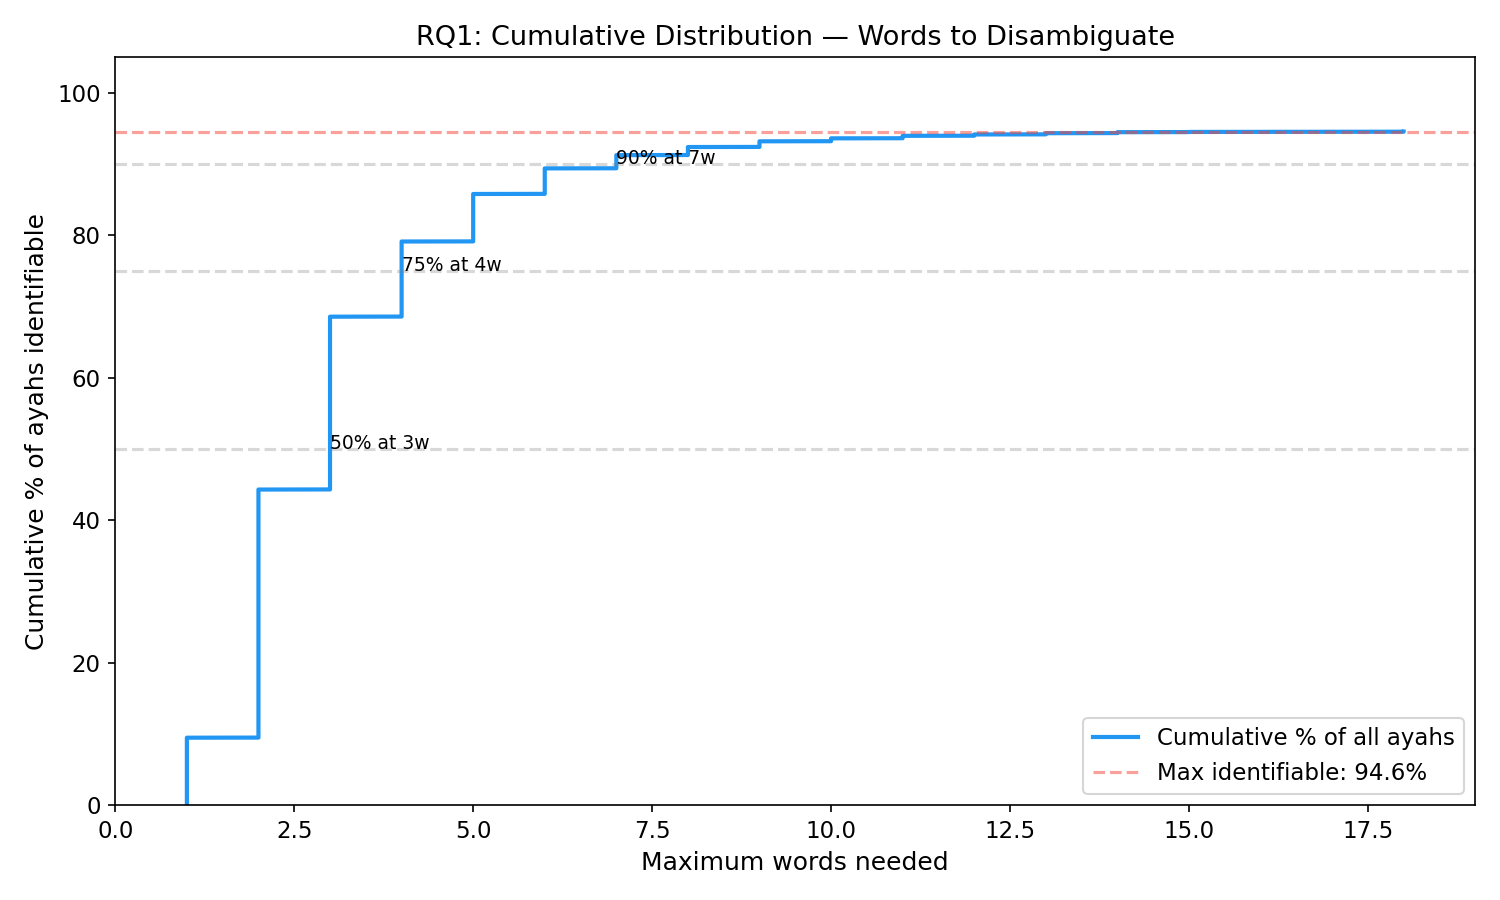
\includegraphics[width=\columnwidth]{fig_01_cdf.png}
  \caption{Cumulative distribution: how quickly ayahs become identifiable from their opening word.}
  \label{fig:cdf}
\end{figure}

\begin{figure}[t]
  \centering
  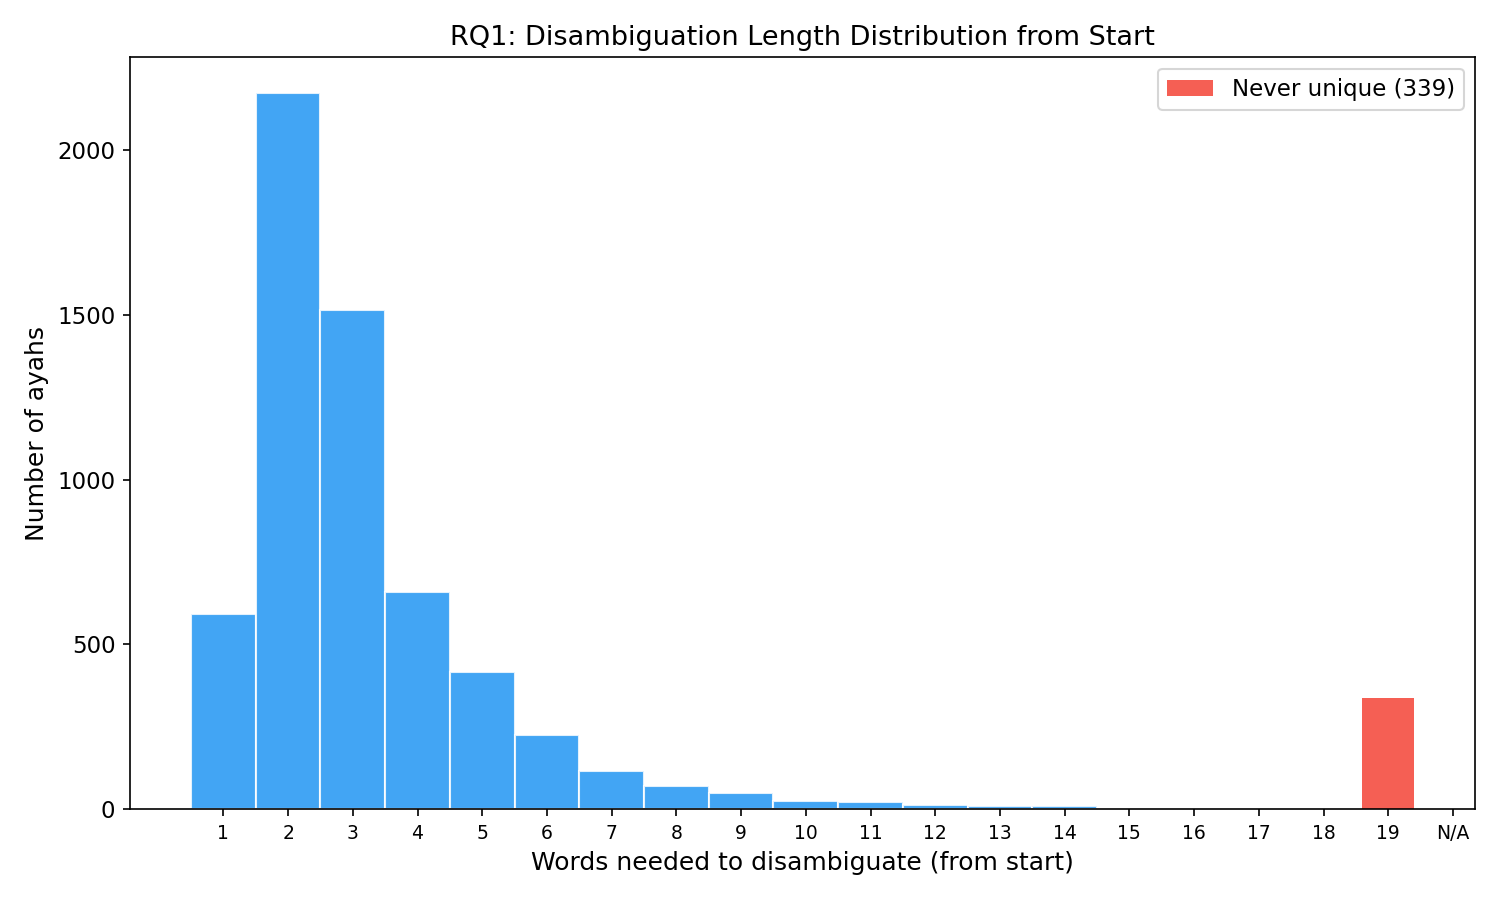
\includegraphics[width=\columnwidth]{fig_02_histogram.png}
  \caption{Distribution of disambiguation lengths from start. The 339 never-unique ayahs are shown in red.}
  \label{fig:histogram}
\end{figure}

592 ayahs are identifiable from their very first word.
Every one of these opens with a hapax legomenon.
The shortest unique openers are just two Arabic characters: \textarabic{سَلْ} (``Ask,'' Q\,2:211), \textarabic{ذُقْ} (``Taste!'' Q\,44:49), and \textarabic{فَكُّ} (``Freeing,'' Q\,90:13).

\subsection{The 339 Never-Unique Ayahs}

339 ayahs cannot be uniquely identified from their start at any length, because their entire text is shared with at least one other ayah.
These cluster into clear structural categories:

\begin{itemize}
  \item \textbf{The basmalah} (Q\,1:1): \textarabic{بِسْمِ ٱللَّهِ ٱلرَّحْمَٰنِ ٱلرَّحِيمِ} appears verbatim at the start of 113 surahs.
  \item \textbf{Surat al-Rahman's refrain} (Q\,55): \textarabic{فَبِأَىِّ ءَالَآءِ رَبِّكُمَا تُكَذِّبَانِ} (``Which of your Lord's favors will you deny?'') is repeated identically 31 times.
  \item \textbf{Surat al-Shu`ara's prophet-narrative phrases} (Q\,26): 53 ayahs share repeated phrases across the surah's seven parallel prophet stories.
  \item \textbf{Al-Saffat} (Q\,37): 28 ayahs. \textbf{Al-Mursalat} (Q\,77): 14 ayahs.
  \item \textbf{Disconnected opening letters} (\emph{\d{h}ur\=uf muqatta`\=at}): e.g., \emph{Alif-L\=am-M\=im} opens six surahs identically.
  \item \textbf{Verbatim-repeated passages}: e.g., Q\,2:134 and Q\,2:141 share all 15 words.
\end{itemize}

However, as we show in \S\ref{sec:boundary}, 328 of these 339 become identifiable when boundary context from the surrounding ayahs is available. Only 11 remain truly unresolvable---and they are fascinating (\S\ref{sec:eleven}).

\subsection{Where in the Ayah Does Identification Happen?}

\begin{figure}[t]
  \centering
  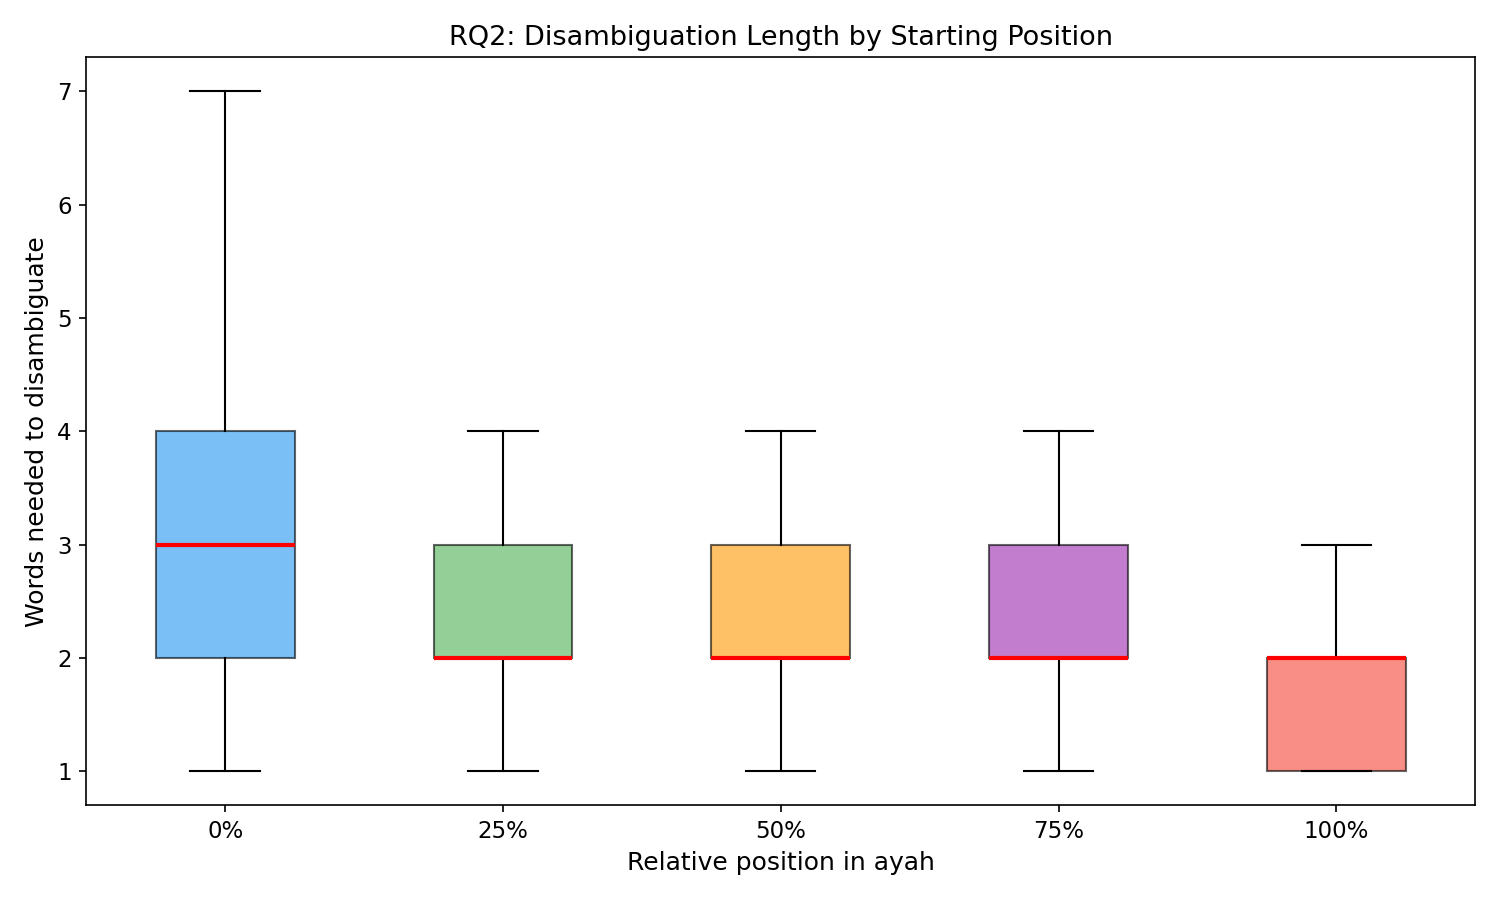
\includegraphics[width=\columnwidth]{fig_03_boxplot.png}
  \caption{Disambiguation length by relative starting position. Endings are systematically easier than beginnings.}
  \label{fig:boxplot}
\end{figure}

Figure~\ref{fig:boxplot} shows a clear pattern: ayah endings are easier to identify than beginnings.
Mean disambiguation drops from 3.22 words at the start to 1.80 at the end.
Openings often share common phrases (\textarabic{يَٰٓأَيُّهَا ٱلَّذِينَ ءَامَنُوا۟} opens 89 ayahs), while closing phrases tend to be more distinctive.

An interesting corollary: for easy ayahs ($d \leq 3$), the disambiguating word falls in the first 20\% of the ayah.
For difficult ayahs ($d \geq 8$), it shifts to the second half (mean: 60\% through the ayah).
The disambiguating word marks the exact boundary between shared and unique content.

\subsection{Surah-Level Patterns}

\begin{figure}[t]
  \centering
  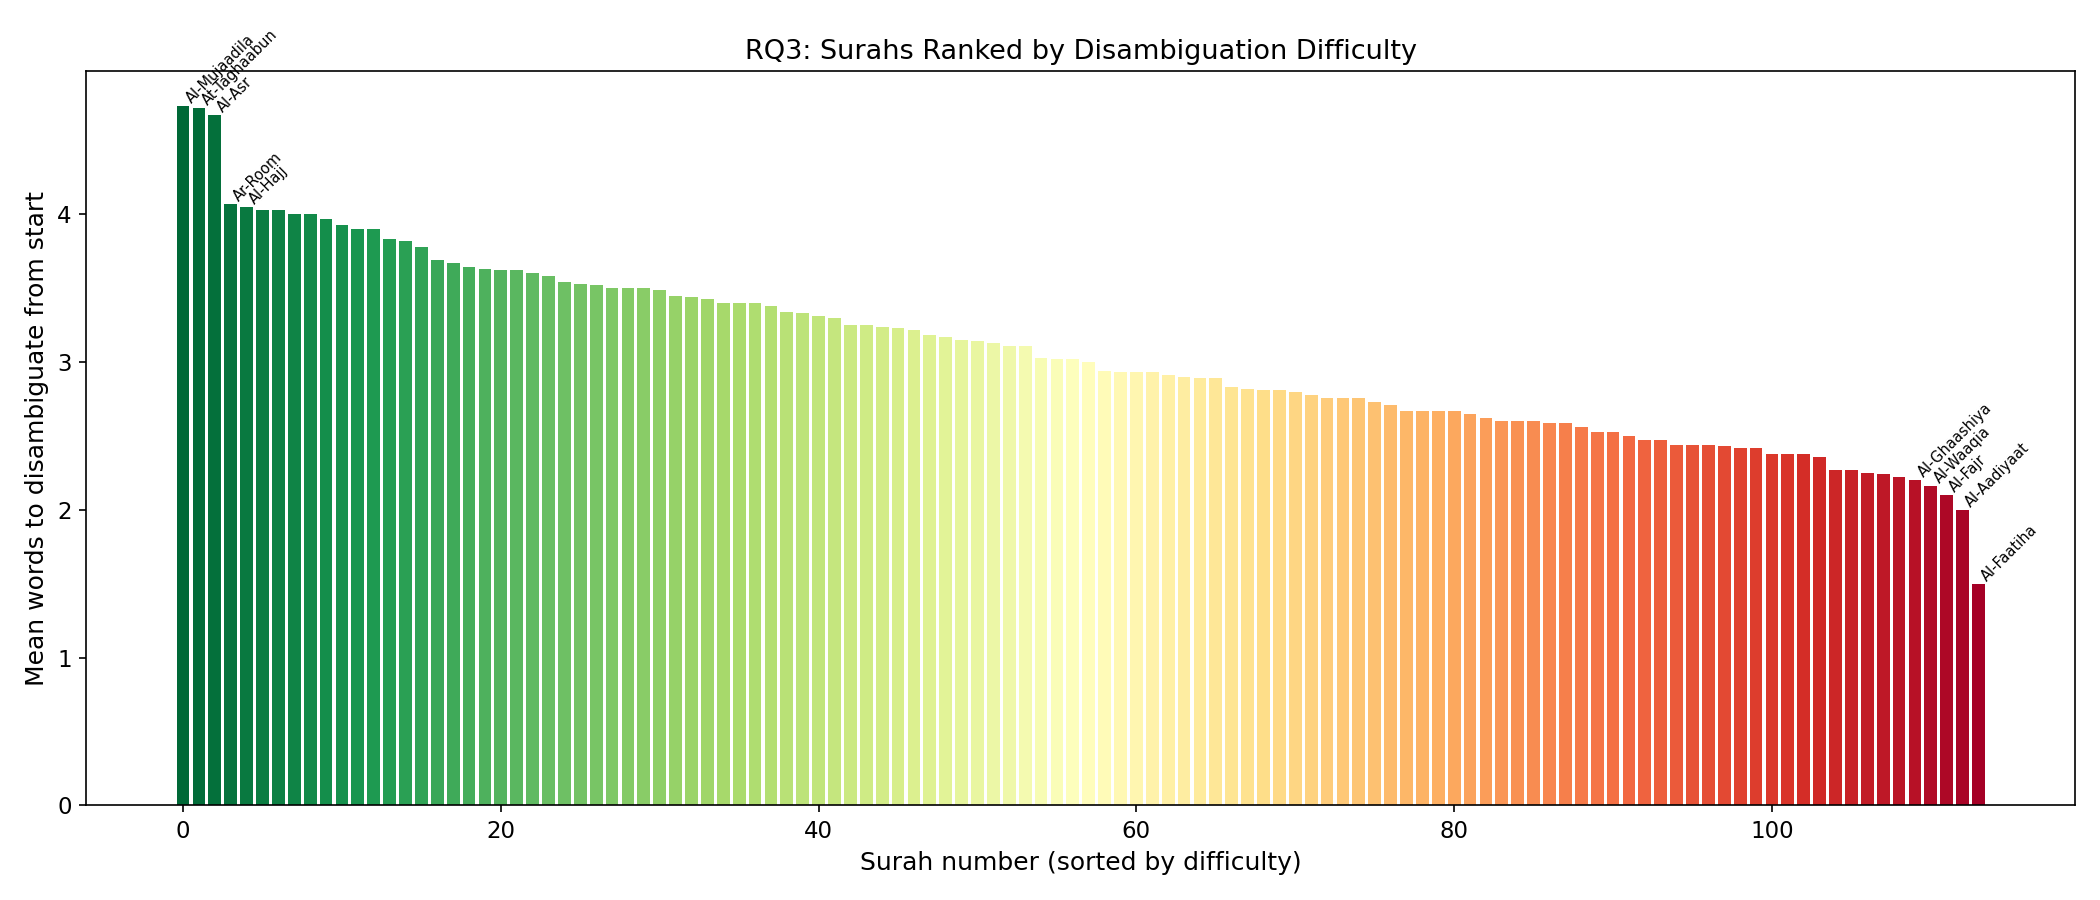
\includegraphics[width=\columnwidth]{fig_04_surah_ranking.png}
  \caption{All 114 surahs ranked by mean disambiguation length.}
  \label{fig:surah_ranking}
\end{figure}

Figure~\ref{fig:surah_ranking} ranks all 114 surahs.
The five requiring the most words: Al-Mujadilah (4.73), Al-Taghabun (4.72), Al-`Asr (4.67), Al-Rum (4.07), and Al-Hajj (4.05).
The easiest: Al-Fatihah (1.50), Al-`Adiyat (2.00), and Al-Fajr (2.10).

\paragraph{Meccan vs.\ Medinan surahs.}
Medinan surahs are systematically harder: mean 3.49 vs.\ 2.98 words (17\% more).
This likely reflects the higher density of shared legislative, theological, and community-oriented vocabulary in the Medinan corpus.

\paragraph{What predicts difficulty?}
The strongest predictor is not ayah length but \emph{vocabulary uniqueness}.
The correlation between a surah's hapax density (fraction of words appearing only once in the Quran) and its mean disambiguation length is $r = -0.54$---a strong negative relationship.
Surahs with more unique vocabulary are substantially easier.
Ayah length, by contrast, correlates only weakly ($r = 0.11$).

\paragraph{Surah heatmaps.}
Figure~\ref{fig:heatmap55} shows the disambiguation ``fingerprint'' of Surat al-Rahman (Q\,55).
The periodic vertical bands correspond to its 31-fold refrain.
Narrative surahs like Yusuf (Q\,12) show uniformly low difficulty (see Appendix~\ref{app:heatmaps}).

\begin{figure}[t]
  \centering
  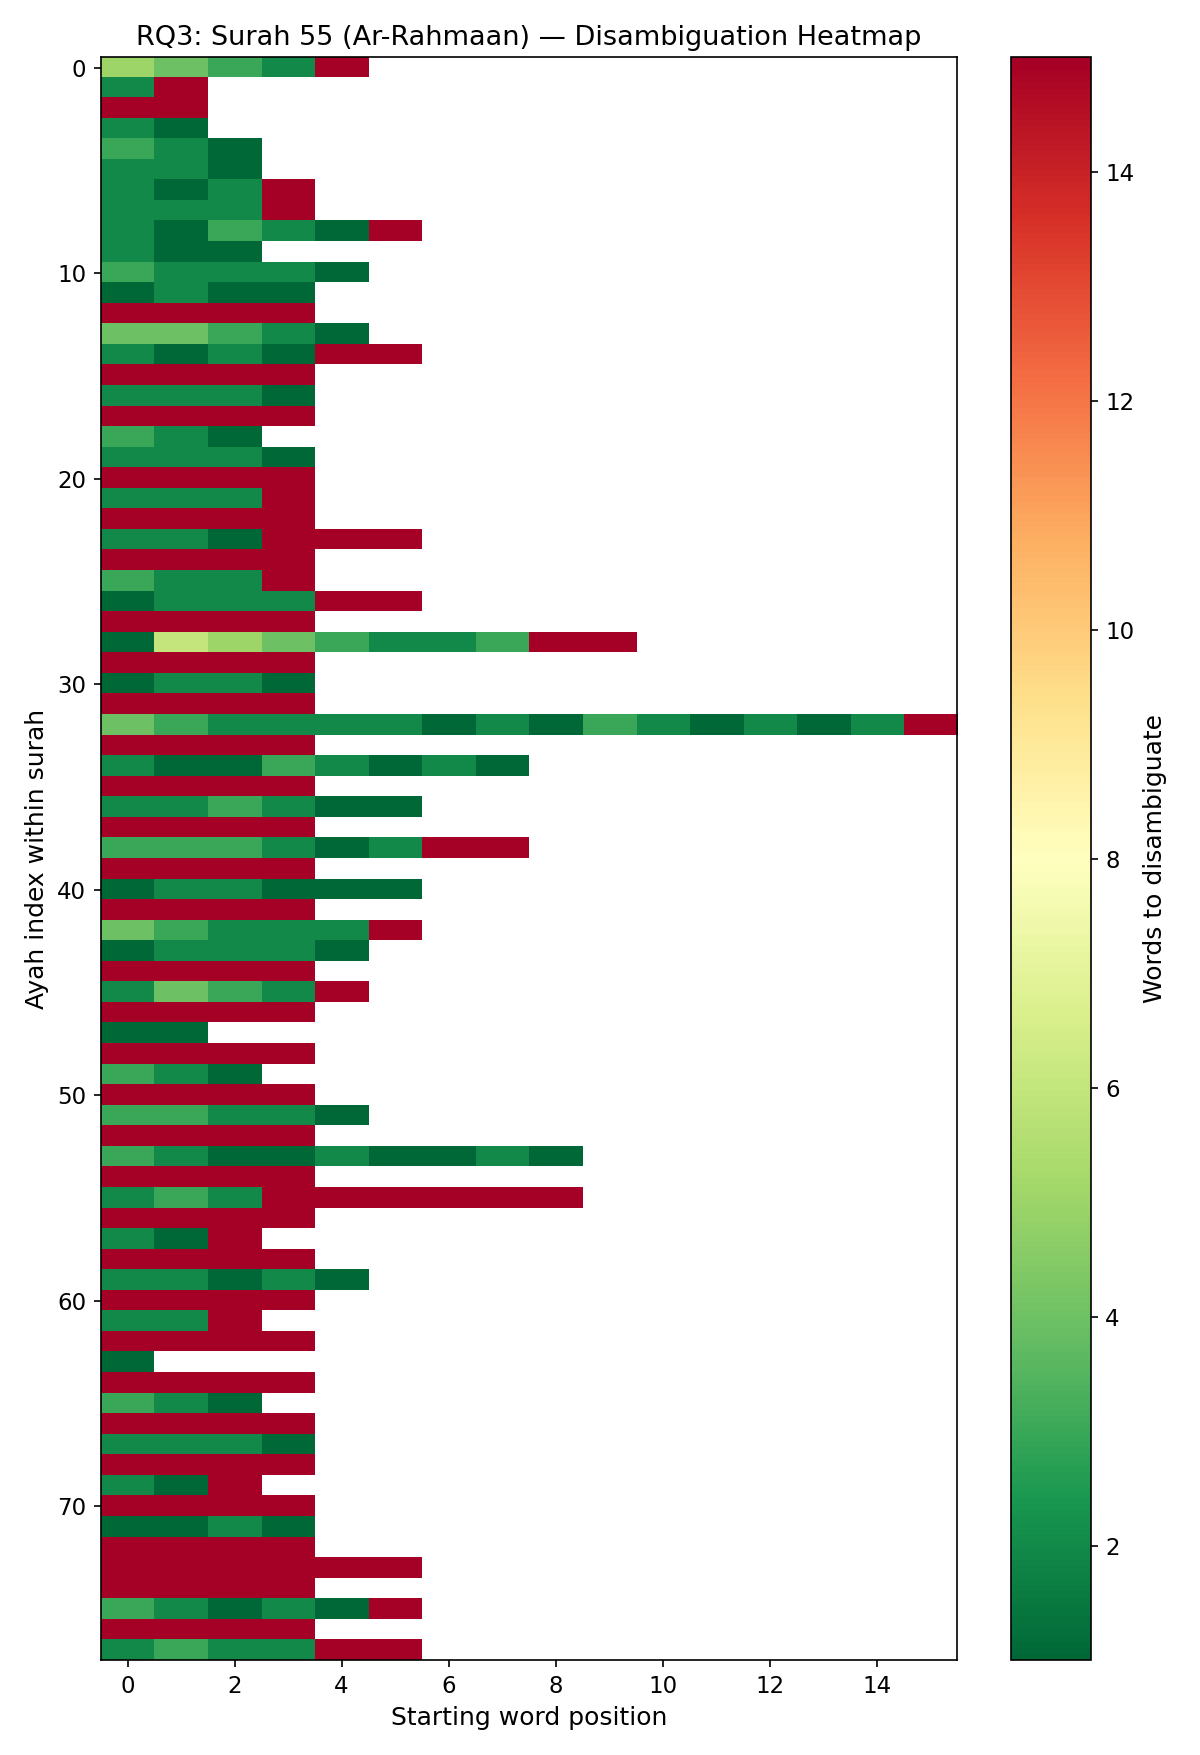
\includegraphics[width=\columnwidth]{fig_05_heatmap_55.png}
  \caption{Surat al-Rahman (Q\,55). Each row is an ayah; each column is a starting position. The vertical bands are the 31-fold refrain.}
  \label{fig:heatmap55}
\end{figure}

\paragraph{By Juz.}
\emph{Huff\=a\d{z}} organize review by \emph{juz'} (one of 30 equal parts).
The easiest is the 27th (mean 2.52), containing many short Meccan surahs.
The most difficult is the 28th (mean 3.88).
Later ajza (parts 16--30) are easier overall than earlier ones (mean 3.09 vs.\ 3.42).

\subsection{Confuser Pairs and Persistent Confusers}

We extract 250{,}482 pairs of ayahs sharing at least one consecutive word.
The longest shared sequence spans \textbf{24 words} between Q\,4:43 and Q\,5:6---both addressing the rulings of ablution and dry purification.

\begin{table}[t]
\centering
\small
\begin{tabular}{llcc}
\toprule
\textbf{Ayah A} & \textbf{Ayah B} & \textbf{Shared} & \textbf{Cross} \\
\midrule
Q\,4:43 & Q\,5:6 & 24 & \checkmark \\
Q\,11:110 & Q\,41:45 & 18 & \checkmark \\
Q\,4:116 & Q\,4:48 & 17 &  \\
Q\,13:25 & Q\,2:27 & 17 & \checkmark \\
Q\,34:2 & Q\,57:4 & 16 & \checkmark \\
Q\,2:134 & Q\,2:141 & 15 &  \\
Q\,59:1 & Q\,61:1 & 15 & \checkmark \\
\bottomrule
\end{tabular}
\caption{Top confuser pairs by shared word-sequence length.}
\label{tab:pairs}
\end{table}

At $\geq$5 shared words, 69.2\% of confuser pairs are cross-surah---a wrong match leads to a completely different location in the text.

\paragraph{Persistent confusers.}
In the trace of Q\,2:14, we saw Q\,2:76 hold on as the single remaining confuser for 6 consecutive words.
We call the last confuser standing in any narrowing curve the \emph{persistent confuser} of that ayah.
886 ayahs (14.2\%) have this ``cliff-then-plateau'' pattern: candidates drop rapidly to a single persistent confuser that holds on for two or more additional words before the ayahs finally diverge.

These relationships are often asymmetric.
Q\,34:2 requires 17 words to distinguish itself from Q\,57:4, but Q\,57:4 needs only 4 words to distinguish itself from Q\,34:2---and its own persistent confuser is Q\,2:29, not Q\,34:2.
677 pairs are \emph{symmetric}: each considers the other its persistent confuser. These are the true twins of the Quran---pairs locked together until the very last distinguishing word.

\paragraph{Confuser graph.}
A graph with edges for pairs sharing $\geq$5 words yields 1{,}821 nodes and 2{,}805 edges across 429 connected components. The largest spans 605 ayahs (Figure~\ref{fig:network}).
The highest-degree hub is Q\,2:255 (\emph{\=Ayat al-Kurs\=i}, 38 connections)---a long, doctrinally rich ayah.
Despite containing 10 of the top 100 repeated phrases, it remains identifiable in 8 words from the start.
Its distinctiveness comes not from unique vocabulary but from the unique \emph{arrangement} of shared building blocks.

\begin{figure}[t]
  \centering
  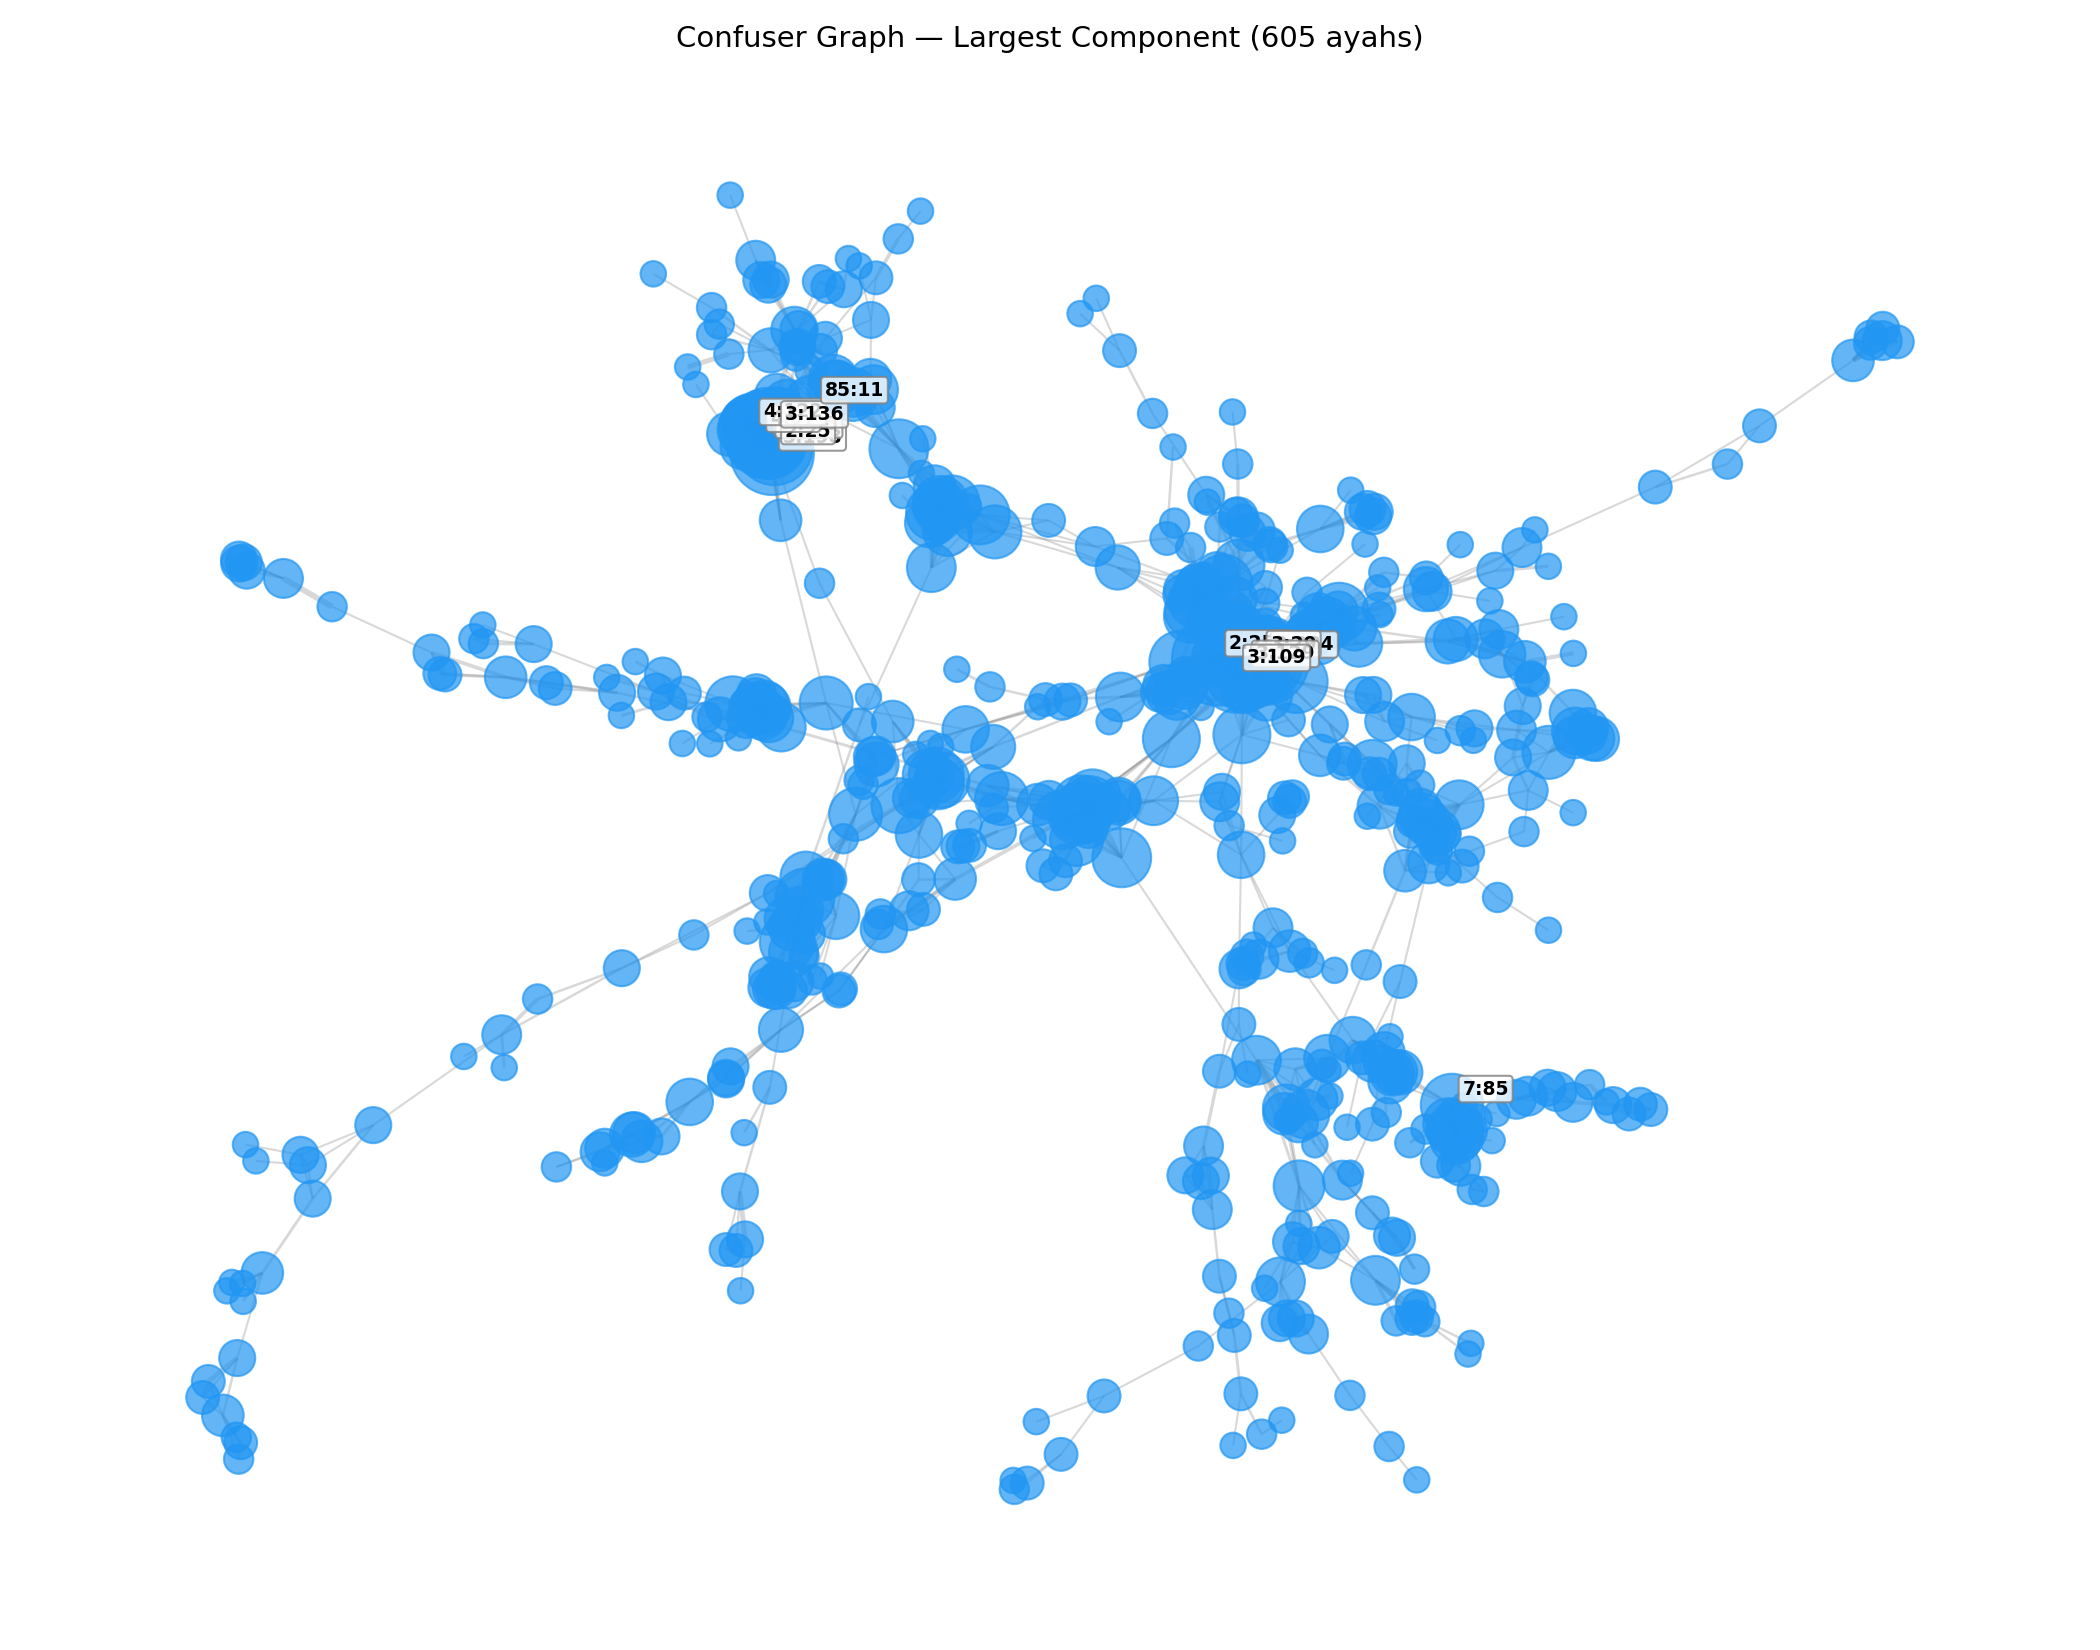
\includegraphics[width=\columnwidth]{fig_06_confuser_network.png}
  \caption{Largest connected component of the confuser graph (605 ayahs).}
  \label{fig:network}
\end{figure}

\subsection{Repeated Phrases}

1{,}957 word sequences appear in five or more distinct ayahs.
The most common: \textarabic{إِنَّ ٱللَّهَ} (``Indeed, God\ldots'') in 243 ayahs, \textarabic{ٱلَّذِينَ ءَامَنُوا۟} (``those who believe'') in 182, and \textarabic{فِى ٱلْأَرْضِ} (``in the earth'') in 170.

The phrases with the highest disambiguation cost are \emph{closing phrases} that appear at the end of many ayahs---because no words follow them, they can never resolve on their own.
\textarabic{غَفُورٌ رَّحِيمٌ} (``Most Forgiving, Most Merciful'') closes 42 ayahs; \textarabic{رَبِّ ٱلْعَٰلَمِينَ} (``Lord of the Worlds'') closes 34.

Some ayahs are composed almost entirely of shared building blocks.
Q\,64:1 and Q\,49:1 achieve 100\% coverage by the top 100 repeated phrases---virtually every word appears as part of a recurring phrase elsewhere.
At the other extreme, surahs like Quraysh (45\% hapax density) and Al-Duha (38.5\%) are built from highly distinctive vocabulary.

\subsection{Continuous Recitation: Cross-Boundary Analysis}
\label{sec:boundary}

The analyses above treat each ayah in isolation.
In practice, recitation is continuous.
We construct the entire Quran as a single 78{,}092-word stream and analyze disambiguation at each of the 6{,}235 ayah boundaries.

For each boundary, we form \emph{crossing windows}: the last $t$ words of the preceding ayah concatenated with the first $h$ words of the next.
We check whether this crossing sequence appears at exactly one position in the continuous stream.

\begin{figure}[t]
  \centering
  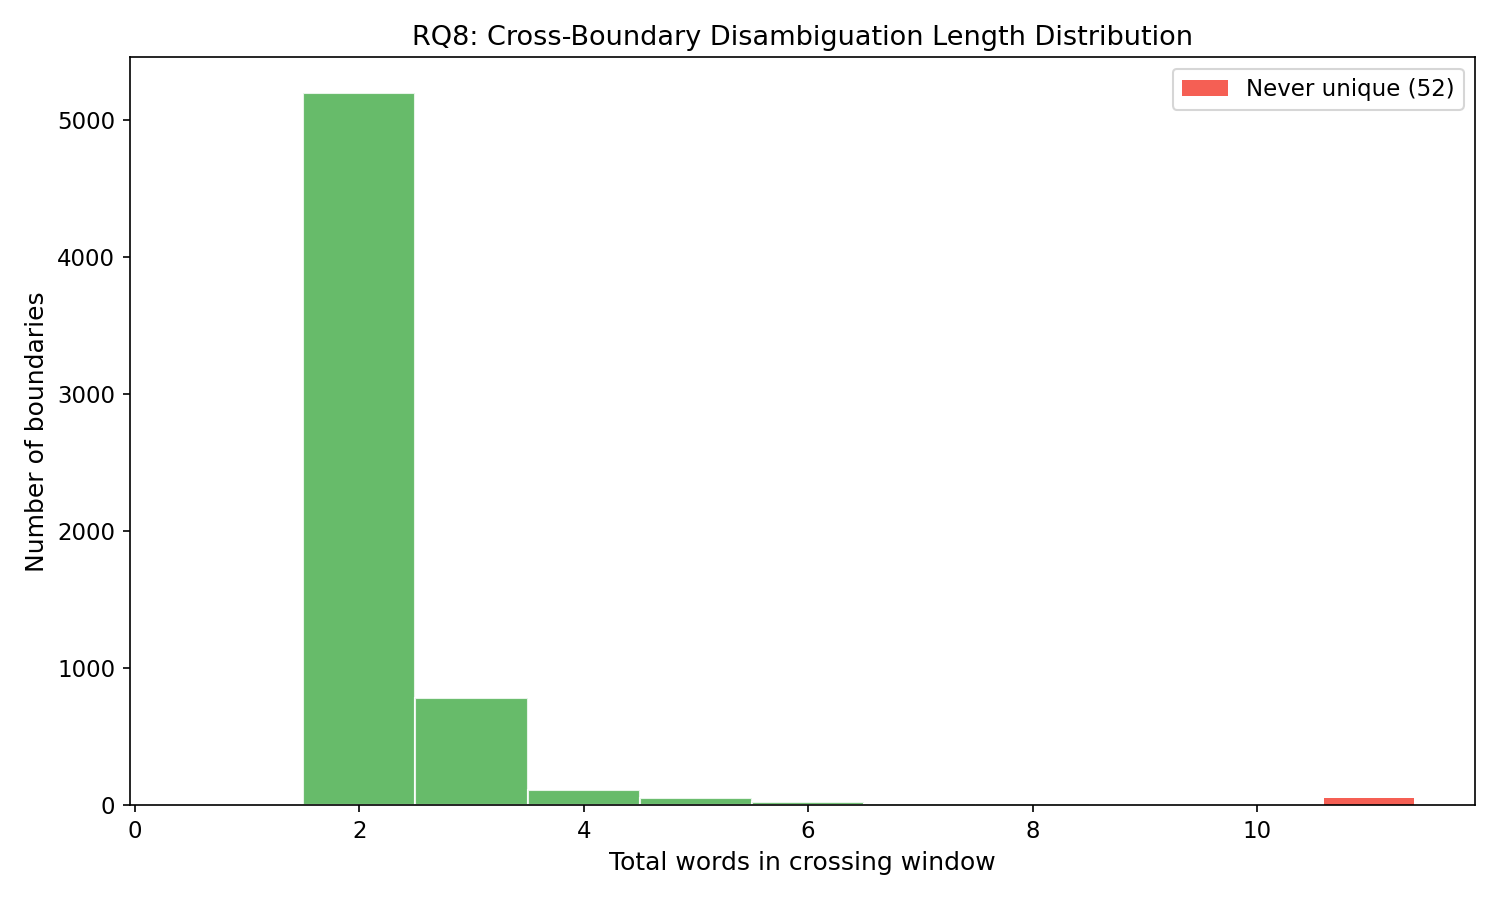
\includegraphics[width=\columnwidth]{fig_08_boundary_histogram.png}
  \caption{Crossing-window lengths at ayah boundaries. Most resolve with just 2 words.}
  \label{fig:boundary_hist}
\end{figure}

The results (Figure~\ref{fig:boundary_hist}): 99.2\% of boundaries are identifiable within 10 words per side, with a mean of 2.22 words (median 2).
Only 52 boundaries remain ambiguous.

\begin{figure}[t]
  \centering
  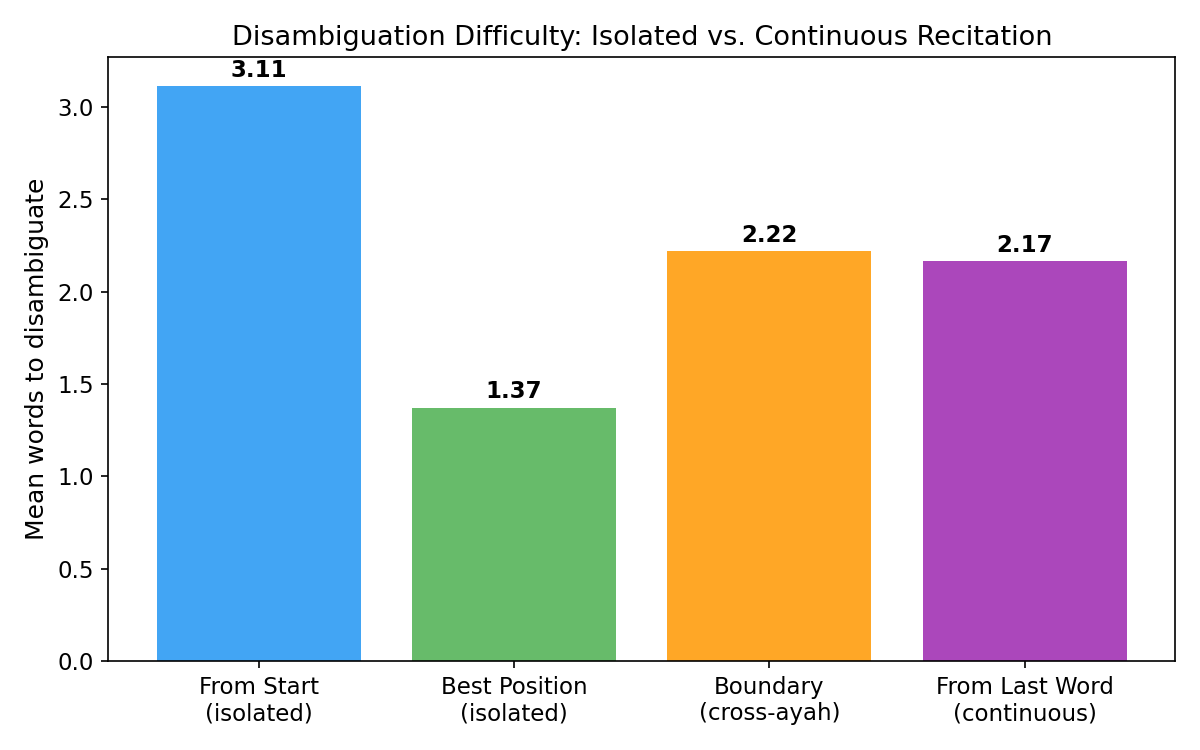
\includegraphics[width=\columnwidth]{fig_09_isolated_vs_boundary.png}
  \caption{Mean disambiguation across four modes.}
  \label{fig:modes}
\end{figure}

The most important finding: of the 339 ayahs that are never unique in isolation, \textbf{328 (96.8\%) become identifiable} with boundary context.
269 of those need just 2 crossing words. 52 need 3--4. Only 7 need 5 or more.

Here are examples of how boundary context resolves otherwise-identical ayahs:

\paragraph{The basmalah.}
Q\,1:1 (\textarabic{بِسْمِ ٱللَّهِ ٱلرَّحْمَٰنِ ٱلرَّحِيمِ}) has 113 confusers---it opens nearly every surah.
But the ayah \emph{after} each basmalah is different: Q\,1:1 is followed by Q\,1:2 (\textarabic{ٱلْحَمْدُ لِلَّهِ رَبِّ ٱلْعَٰلَمِينَ}), while Q\,2's basmalah is followed by Q\,2:2 (\textarabic{ذَٰلِكَ ٱلْكِتَٰبُ}). One word across the boundary is enough.

\paragraph{Al-Rahman's refrain.}
All 31 instances of \textarabic{فَبِأَىِّ ءَالَآءِ رَبِّكُمَا تُكَذِّبَانِ} are identical---but each is preceded and followed by a different ayah.
Q\,55:13 is preceded by Q\,55:12 (about the two types of grain) and followed by Q\,55:14 (creation from clay).
Q\,55:16 is preceded by Q\,55:15 (creation from fire).
Just 2 crossing words resolve all 31 instances.

\paragraph{Verbatim twins.}
Q\,2:134 and Q\,2:141 share all 15 words (\textarabic{تِلْكَ أُمَّةٌ قَدْ خَلَتْ\ldots}).
But Q\,2:134 is preceded by Q\,2:133 (about the testament of Ya`qub, peace be upon him) and Q\,2:141 is preceded by Q\,2:140 (about claiming prophets' religious affiliation). Two crossing words resolve the pair.

\subsection{The 11 Truly Unresolvable Ayahs}
\label{sec:eleven}

Only 11 ayahs in the entire Quran remain unidentifiable even with boundary context.
What makes them special is not just that they are repeated---but that their \emph{neighbors} are also repeated in the same pattern.
The ayah, the ayah before it, and the ayah after it all appear identically at another location, creating a sequence of three or more consecutive shared ayahs.

Here is the complete list, traced to show why boundary context fails:

\begin{algorithm}[H]
\caption{Q\,26:108 --- ``So be mindful of God and obey me'' (also Q\,26:126, 26:144, 26:163, 26:179)}
\label{alg:stuck1}
\smallskip
\centering
\begin{tabular}{@{}l l l@{}}
\toprule
\textbf{Position} & \textbf{Ayah} & \textbf{Status} \\
\midrule
Before & Q\,26:107: \textarabic{إِنِّى لَكُمْ رَسُولٌ أَمِينٌ} & Also repeated 5$\times$ \\
\textbf{This} & \textbf{Q\,26:108}: \textarabic{فَٱتَّقُوا۟ ٱللَّهَ وَأَطِيعُونِ} & \textbf{Repeated 5$\times$} \\
After & Q\,26:109: \textarabic{وَمَآ أَسْـَٔلُكُمْ عَلَيْهِ مِنْ أَجْرٍ\ldots} & Also repeated 5$\times$ \\
\bottomrule
\end{tabular}
\smallskip

\raggedright
In Surat al-Shu`ara' (Q\,26), five prophets each deliver the same three-ayah sequence: ``I am a trustworthy messenger to you / So be mindful of God and obey me / I ask no reward from you\ldots'' This entire block---before, during, and after---repeats identically five times (at ayahs 107--109, 125--127, 143--145, 162--164, 178--180). No amount of local context can distinguish which prophet's story is being recited.
\end{algorithm}

\begin{algorithm}[H]
\caption{Q\,15:37 and Q\,38:80 --- ``He said: You are among those given respite''}
\label{alg:stuck2}
\smallskip
\centering
\begin{tabular}{@{}l l l@{}}
\toprule
\textbf{Position} & \textbf{Q\,15:37} & \textbf{Q\,38:80} \\
\midrule
Before & Q\,15:36: \textarabic{قَالَ رَبِّ فَأَنظِرْنِىٓ\ldots} & Q\,38:79: same text \\
\textbf{This} & \textarabic{قَالَ فَإِنَّكَ مِنَ ٱلْمُنظَرِينَ} & same text \\
After & Q\,15:38: \textarabic{إِلَىٰ يَوْمِ ٱلْوَقْتِ ٱلْمَعْلُومِ} & Q\,38:81: same text \\
\bottomrule
\end{tabular}
\smallskip

\raggedright
The exchange between God and Iblis about being granted respite appears in both Surat al-Hijr and Surat Sad with identical wording across three consecutive ayahs.
\end{algorithm}

\begin{algorithm}[H]
\caption{Q\,23:6--7 and Q\,70:30--31 --- Two consecutive shared ayahs}
\label{alg:stuck3}
\smallskip
\centering
\begin{tabular}{@{}l l l@{}}
\toprule
\textbf{Position} & \textbf{Q\,23:6--7} & \textbf{Q\,70:30--31} \\
\midrule
Before & Q\,23:5: same as Q\,70:29 & Q\,70:29: same as Q\,23:5 \\
\textbf{23:6/70:30} & \textarabic{إِلَّا عَلَىٰٓ أَزْوَٰجِهِمْ\ldots} & same text (10 words) \\
\textbf{23:7/70:31} & \textarabic{فَمَنِ ٱبْتَغَىٰ وَرَآءَ ذَٰلِكَ\ldots} & same text (7 words) \\
After & Q\,23:8: same as Q\,70:32 & Q\,70:32: same as Q\,23:8 \\
\bottomrule
\end{tabular}
\smallskip

\raggedright
Surat al-Mu'minun and Surat al-Ma`arij both contain a passage about the believers' qualities, with four consecutive ayahs shared verbatim between the two surahs (Q\,23:5--8 $\leftrightarrow$ Q\,70:29--32).
\end{algorithm}

\medskip

The pattern is consistent: all 11 unresolvable ayahs are embedded in \emph{runs} of consecutive shared ayahs---sequences where not just the ayah itself but its entire local neighborhood is duplicated elsewhere.
Five are from Al-Shu`ara' (the prophet-narrative refrain), two from the Iblis dialogue (Al-Hijr/Sad), two from Al-Mu'minun, and two from Al-Ma`arij.

To resolve these, a system would need context extending \emph{beyond} the immediate neighbors---essentially knowing which surah is currently being recited.
In continuous recitation, this context is always available from earlier in the recitation.

% ============================================================================
\section{Structural Indexing}
\label{sec:indexing}

\paragraph{Minimum index depth.}
An index of all 25-grams suffices to uniquely fingerprint every ayah from at least one starting position.

\paragraph{Identifiability frontier.}
Figure~\ref{fig:frontier} shows the fraction of ayahs identifiable as a function of $n$-gram size.
At $n{=}1$: 9.5\%.
At $n{=}3$: 68.6\%.
At $n{=}6$: 89.4\%.
The curve plateaus near 94.6\%.

\begin{figure}[t]
  \centering
  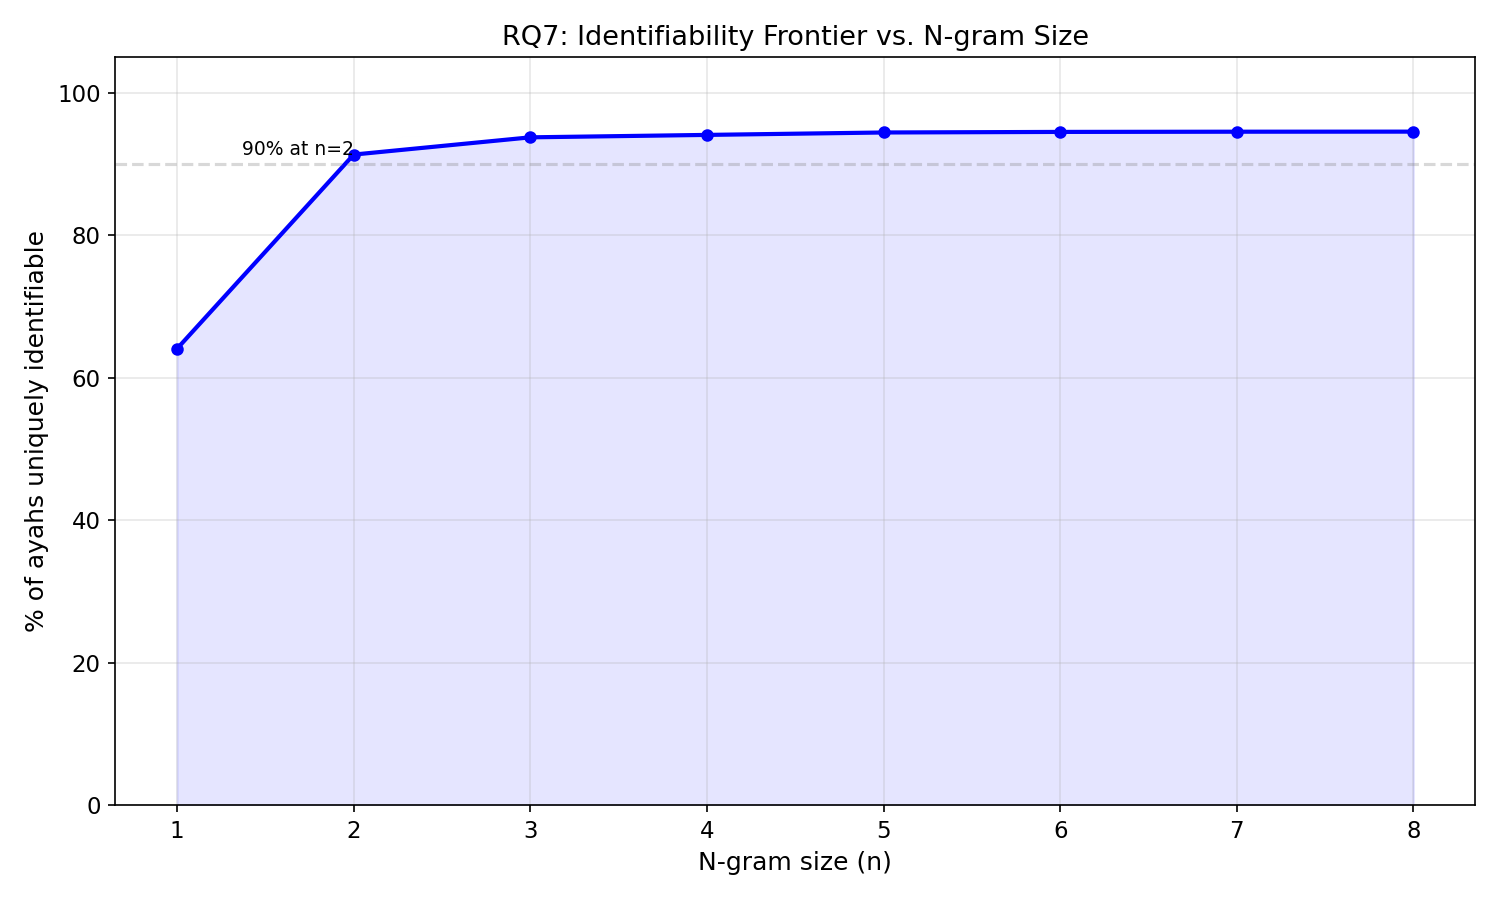
\includegraphics[width=\columnwidth]{fig_07_identifiability.png}
  \caption{Fraction of ayahs identifiable vs.\ $n$-gram size.}
  \label{fig:frontier}
\end{figure}

\paragraph{Fingerprint set.}
The shortest unique identifying substring per ayah has a mean of 1.37 words (median 1).
39.4\% of ayahs achieve their shortest fingerprint from a non-initial position---a prefix-only index would miss these.

% ============================================================================
\section{What This Data Enables}
\label{sec:enables}

We release this dataset in the hope that others will find uses for it we have not considered. Some directions we think are worth exploring:

\paragraph{Phonemic disambiguation.}
Our analysis is purely orthographic.
Two ayahs that differ in spelling can sound nearly identical under \emph{tajw\=id} rules, and similar-looking ayahs may sound quite different.
A tajw\=id-aware phonemic layer---mapping text to IPA sequences---would capture a complementary dimension.
We believe this is the highest-value extension.

\paragraph{Jump recovery.}
When a system commits to the wrong ayah at a shared phrase, how many additional words before the error becomes detectable?
Our data could support such analysis, but the combinatorial space is large.

\paragraph{ASR confidence.}
The disambiguation map provides, at any word position, the number of candidate ayahs still in play.
This could serve as a confidence signal for speech recognition systems.

\paragraph{Qira'at sensitivity.}
Our analysis uses the Hafs reading.
How does the map change across the seven canonical readings?

\paragraph{Correlation with tafsir.}
Do the confuser clusters align with thematic groupings recognized in classical \emph{tafs\=ir}?
The 11-ayah clique around cosmological declarations suggests such connections may exist.

\paragraph{Adaptive systems.}
Could a recitation-assistance system use the narrowing curves to provide real-time feedback---waiting to commit until enough words have been heard, and indicating when a high-ambiguity region begins?

% ============================================================================
\section{Limitations}
\label{sec:limitations}

This analysis operates on normalized orthographic forms only.
It does not model phonemic similarity, morphological variation, or contextual meaning.
Whitespace tokenization treats Arabic proclitics as part of their attached token; stem-aware matching changes disambiguation for approximately 26\% of windows, with a modest overall increase (mean 2.74 to 2.85), confirming robustness while highlighting proclitic-aware tokenization as a refinement.

The cross-boundary model uses a fixed 10-word context window.
A system mid-stream has the entire prior context, making our analysis conservative.

We make no claims about the memorization tradition.
The Quran has been memorized by millions of people across 14 centuries, and the challenge of similar passages has been addressed by scholars far more qualified than us.
This is a computational tool, nothing more.

% ============================================================================
\section{Conclusion}

We present a complete disambiguation map of the Quran: for every ayah, at every word position, how many words until identification is unique.
The method is parameter-free, deterministic, and runs in 6.5 seconds.
The median ayah is identifiable within 3 words.
Under continuous recitation, 96.8\% of never-unique ayahs become resolvable, leaving only 11 truly unresolvable ayahs---all embedded in runs of consecutive shared passages.
The strongest predictor of a surah's disambiguation difficulty is its proportion of unique vocabulary ($r = -0.54$), not its length.

We release six JSON artifacts (77\,MB) under CC BY 4.0, along with all source code.
We hope this resource proves useful, and that it serves, however modestly, the broader effort to develop respectful, high-quality tools for engaging with the Quran.

\emph{Wa All\=ahu a`lam} (And God knows best).

% ============================================================================
\bibliographystyle{plainnat}
\bibliography{references}

% ============================================================================
\clearpage
\appendix

\section{Dataset Artifacts}
\label{app:datasets}

\begin{table}[h]
\centering
\small
\begin{tabular}{lrl}
\toprule
\textbf{File} & \textbf{Size} & \textbf{Description} \\
\midrule
\texttt{disambiguation-map.json} & 69\,MB & Full per-ayah, per-position \\
 & & narrowing curves \\
\texttt{disambiguation-compact.json} & 619\,KB & Lightweight: $d[\,]$ per ayah \\
\texttt{fingerprints.json} & 591\,KB & Shortest unique substring \\
 & & per ayah \\
\texttt{confuser-pairs.json} & 32\,KB & Top 500 pairs by \\
 & & shared length \\
\texttt{shared-phrases.json} & 15\,KB & 200 most-repeated \\
 & & word sequences \\
\texttt{boundary-analysis.json} & 2.5\,MB & Cross-boundary \\
 & & disambiguation \\
\bottomrule
\end{tabular}
\caption{Released dataset artifacts.}
\label{tab:artifacts}
\end{table}

\section{Never-Unique Ayah Categories}
\label{app:never_unique}

\begin{table}[h]
\centering
\small
\begin{tabular}{lrc}
\toprule
\textbf{Category} & \textbf{Count} & \textbf{Example} \\
\midrule
Basmalah & 113+ & Q\,1:1 \\
Al-Ra\d{h}m\=an refrain & 31 & Q\,55:13--77 \\
Al-Shu`ar\=a' shared phrases & 53 & Q\,26:8--191 \\
Al-\d{S}\=aff\=at shared phrases & 28 & Q\,37:40--182 \\
Al-Mursal\=at refrain & 14 & Q\,77:15--50 \\
Al-\d{H}ijr shared phrases & 14 & Q\,15:29--93 \\
\d{S}\=ad shared phrases & 10 & Q\,38:3--87 \\
\d{H}ur\=uf muqatta`\=at & 8 & Q\,2:1 \\
Other verbatim repeats & 58 & Q\,2:134/141 \\
\bottomrule
\end{tabular}
\caption{The 339 never-unique ayahs by category.}
\label{tab:never_unique_cats}
\end{table}

\section{Never-Unique Boundary Categories}
\label{app:never_unique_boundaries}

\begin{table}[h]
\centering
\small
\begin{tabular}{rlcl}
\toprule
\textbf{\#} & \textbf{Surah} & \textbf{Count} & \textbf{Cause} \\
\midrule
26 & Al-Shu`ar\=a' & 20 & Prophet-narrative refrain \\
37 & Al-\d{S}\=aff\=at & 4 & ``Sal\=amun `al\=a'' phrases \\
15 & Al-\d{H}ijr & 4 & ``Inn\=a la-na\d{h}nu'' refrain \\
23 & Al-Mu'min\=un & 3 & Shared passage \\
38 & \d{S}\=ad & 3 & Prophet-narrative echoes \\
70 & Al-Ma`\=arij & 3 & Shared passage \\
\midrule
\multicolumn{2}{l}{\emph{11 other surahs}} & 15 & 1--2 each \\
\bottomrule
\end{tabular}
\caption{The 52 never-unique boundaries by surah.}
\label{tab:never_unique_boundaries}
\end{table}

\section{All 114 Surahs}
\label{app:surah_table}

\begin{table}[h]
\centering
\scriptsize
\setlength{\tabcolsep}{2pt}
\begin{minipage}[t]{0.48\textwidth}
\centering
\begin{tabular}{rl r r r r r lr}
\toprule
\textbf{\#} & \textbf{Surah} & \textbf{Ay.} & \textbf{Mean} & \textbf{Med.} & \textbf{NU} & \textbf{Best} & \textbf{Hardest} & \textbf{$d$} \\
\midrule
1 & Al-F\=ati\d{h}ah & 7 & 1.50 & 1.5 & 3 & 1.25 & 1:4 & 2 \\
2 & Al-Baqarah & 286 & 3.78 & 3.0 & 8 & 1.35 & 2:48 & 12 \\
3 & \=Al-i-`Imr\=an & 200 & 3.34 & 3.0 & 5 & 1.36 & 3:10 & 14 \\
4 & Al-Nis\=a' & 176 & 3.52 & 3.0 & 0 & 1.28 & 4:48 & 18 \\
5 & Al-M\=a'idah & 120 & 3.64 & 3.0 & 2 & 1.27 & 5:17 & 11 \\
6 & Al-An`\=am & 165 & 3.63 & 3.0 & 3 & 1.35 & 6:152 & 13 \\
7 & Al-A`r\=af & 206 & 3.44 & 3.0 & 7 & 1.35 & 7:54 & 15 \\
8 & Al-Anf\=al & 75 & 3.43 & 3.0 & 0 & 1.32 & 8:39 & 8 \\
9 & Al-Tawbah & 129 & 2.76 & 2.0 & 2 & 1.21 & 9:11 & 7 \\
10 & Y\=unus & 109 & 3.60 & 3.0 & 2 & 1.60 & 10:3 & 15 \\
11 & H\=ud & 123 & 3.49 & 3.0 & 2 & 1.30 & 11:50 & 14 \\
12 & Y\=usuf & 111 & 2.93 & 3.0 & 0 & 1.19 & 12:102 & 11 \\
13 & Al-Ra`d & 43 & 3.53 & 3.0 & 0 & 1.35 & 13:7 & 10 \\
14 & Ibr\=ah\=im & 52 & 3.02 & 3.0 & 1 & 1.25 & 14:2 & 10 \\
15 & Al-\d{H}ijr & 99 & 3.13 & 3.0 & 14 & 1.52 & 15:19 & 10 \\
16 & Al-Na\d{h}l & 128 & 3.40 & 3.0 & 2 & 1.58 & 16:115 & 10 \\
17 & Al-Isr\=a' & 111 & 3.25 & 3.0 & 1 & 1.22 & 17:34 & 13 \\
18 & Al-Kahf & 110 & 2.91 & 2.0 & 2 & 1.15 & 18:110 & 12 \\
19 & Maryam & 98 & 3.02 & 2.0 & 1 & 1.26 & 19:10 & 11 \\
20 & \d{T}\=a H\=a & 135 & 2.80 & 2.0 & 2 & 1.32 & 20:71 & 13 \\
21 & Al-Anbiy\=a' & 112 & 2.81 & 3.0 & 2 & 1.39 & 21:28 & 8 \\
22 & Al-\d{H}ajj & 78 & 4.05 & 3.0 & 1 & 1.36 & 22:14 & 13 \\
23 & Al-Mu'min\=un & 118 & 3.11 & 3.0 & 9 & 1.58 & 23:21 & 9 \\
24 & Al-N\=ur & 64 & 3.38 & 3.0 & 1 & 1.32 & 24:61 & 13 \\
25 & Al-Furq\=an & 77 & 3.17 & 3.0 & 1 & 1.25 & 25:59 & 14 \\
26 & Al-Shu`ar\=a' & 227 & 2.67 & 2.0 & 53 & 1.52 & 26:49 & 13 \\
27 & Al-Naml & 93 & 2.93 & 3.0 & 3 & 1.40 & 27:69 & 9 \\
28 & Al-Qa\d{s}a\d{s} & 88 & 2.89 & 3.0 & 4 & 1.32 & 28:48 & 7 \\
29 & Al-`Ankab\=ut & 69 & 3.69 & 3.0 & 2 & 1.37 & 29:68 & 10 \\
30 & Al-R\=um & 60 & 4.07 & 4.0 & 2 & 1.48 & 30:9 & 12 \\
31 & Luqm\=an & 34 & 3.93 & 3.0 & 4 & 1.50 & 31:21 & 12 \\
32 & Al-Sajdah & 30 & 3.14 & 3.0 & 1 & 1.59 & 32:22 & 7 \\
33 & Al-A\d{h}z\=ab & 73 & 2.94 & 3.0 & 1 & 1.32 & 33:62 & 8 \\
34 & Saba' & 54 & 3.58 & 3.0 & 1 & 1.36 & 34:2 & 17 \\
35 & F\=a\d{t}ir & 45 & 3.90 & 3.0 & 3 & 1.33 & 35:13 & 14 \\
36 & Y\=a S\=in & 83 & 2.76 & 3.0 & 3 & 1.44 & 36:29 & 8 \\
37 & Al-\d{S}\=aff\=at & 182 & 2.38 & 2.0 & 28 & 1.58 & 37:53 & 7 \\
38 & \d{S}\=ad & 88 & 2.82 & 3.0 & 10 & 1.26 & 38:3 & 7 \\
39 & Al-Zumar & 75 & 3.45 & 3.0 & 2 & 1.41 & 39:27 & 10 \\
40 & Gh\=afir & 85 & 3.22 & 3.0 & 3 & 1.48 & 40:82 & 12 \\
41 & Fu\d{s}\d{s}ilat & 54 & 3.50 & 3.0 & 2 & 1.58 & 41:6 & 12 \\
42 & Al-Sh\=ur\=a & 53 & 3.15 & 3.0 & 1 & 1.35 & 42:4 & 8 \\
43 & Al-Zukhruf & 89 & 2.65 & 2.0 & 3 & 1.45 & 43:9 & 8 \\
44 & Al-Dukh\=an & 59 & 2.71 & 2.0 & 4 & 1.60 & 44:8 & 7 \\
45 & Al-J\=athiyah & 37 & 3.23 & 3.0 & 2 & 1.54 & 45:15 & 8 \\
46 & Al-A\d{h}q\=af & 35 & 4.03 & 3.0 & 2 & 1.39 & 46:7 & 9 \\
47 & Mu\d{h}ammad & 38 & 3.97 & 3.5 & 0 & 1.26 & 47:12 & 13 \\
48 & Al-Fat\d{h} & 29 & 3.54 & 3.0 & 1 & 1.43 & 48:17 & 13 \\
49 & Al-\d{H}ujur\=at & 18 & 3.83 & 3.0 & 0 & 1.22 & 49:1 & 9 \\
50 & Q\=af & 45 & 3.31 & 3.0 & 0 & 1.47 & 50:39 & 12 \\
51 & Al-Dh\=ariy\=at & 60 & 2.47 & 2.0 & 2 & 1.47 & 51:25 & 7 \\
52 & Al-\d{T}\=ur & 49 & 2.67 & 2.0 & 4 & 1.38 & 52:1 & 5 \\
53 & Al-Najm & 62 & 2.42 & 2.0 & 0 & 1.35 & 53:31 & 8 \\
54 & Al-Qamar & 55 & 2.47 & 2.0 & 8 & 1.30 & 54:1 & 5 \\
55 & Al-Ra\d{h}m\=an & 78 & 2.22 & 2.0 & 33 & 1.22 & 55:1 & 5 \\
56 & Al-W\=aqi`ah & 96 & 2.16 & 2.0 & 10 & 1.33 & 56:1 & 6 \\
57 & Al-\d{H}ad\=id & 29 & 4.03 & 4.0 & 0 & 1.62 & 57:1 & 10 \\
\bottomrule
\end{tabular}
\end{minipage}%
\hfill
\begin{minipage}[t]{0.48\textwidth}
\centering
\begin{tabular}{rl r r r r r lr}
\toprule
\textbf{\#} & \textbf{Surah} & \textbf{Ay.} & \textbf{Mean} & \textbf{Med.} & \textbf{NU} & \textbf{Best} & \textbf{Hardest} & \textbf{$d$} \\
\midrule
58 & Al-Muj\=adilah & 22 & 4.73 & 5.0 & 0 & 1.27 & 58:17 & 10 \\
59 & Al-\d{H}ashr & 24 & 3.30 & 2.0 & 1 & 1.22 & 59:22 & 8 \\
60 & Al-Mumta\d{h}anah & 13 & 3.62 & 3.0 & 0 & 1.23 & 60:1 & 9 \\
61 & Al-\d{S}aff & 14 & 4.00 & 4.0 & 2 & 1.33 & 61:7 & 7 \\
62 & Al-Jumu`ah & 11 & 3.90 & 3.0 & 1 & 1.50 & 62:1 & 13 \\
63 & Al-Mun\=afiq\=un & 11 & 3.82 & 3.0 & 0 & 1.18 & 63:2 & 8 \\
64 & Al-Tagh\=abun & 18 & 4.72 & 5.0 & 0 & 1.72 & 64:1 & 13 \\
65 & Al-\d{T}al\=aq & 12 & 3.00 & 2.5 & 0 & 1.08 & 65:1 & 7 \\
66 & Al-Ta\d{h}r\=im & 12 & 3.18 & 3.0 & 1 & 1.09 & 66:1 & 7 \\
67 & Al-Mulk & 30 & 3.03 & 3.0 & 1 & 1.38 & 67:1 & 5 \\
68 & Al-Qalam & 52 & 2.38 & 2.0 & 7 & 1.36 & 68:1 & 5 \\
69 & Al-\d{H}\=aqqah & 52 & 2.44 & 2.0 & 7 & 1.31 & 69:19 & 6 \\
70 & Al-Ma`\=arij & 44 & 2.59 & 2.0 & 7 & 1.51 & 70:1 & 5 \\
71 & N\=u\d{h} & 28 & 2.78 & 2.0 & 1 & 1.26 & 71:1 & 6 \\
72 & Al-Jinn & 28 & 2.89 & 3.0 & 0 & 1.29 & 72:1 & 6 \\
73 & Al-Muzzammil & 20 & 2.53 & 2.0 & 1 & 1.26 & 73:1 & 6 \\
74 & Al-Muddaththir & 56 & 2.27 & 2.0 & 1 & 1.36 & 74:1 & 6 \\
75 & Al-Qiy\=amah & 40 & 2.44 & 2.0 & 1 & 1.31 & 75:1 & 7 \\
76 & Al-Ins\=an & 31 & 2.93 & 3.0 & 1 & 1.20 & 76:30 & 7 \\
77 & Al-Mursal\=at & 50 & 2.44 & 2.0 & 14 & 1.33 & 77:1 & 5 \\
78 & Al-Naba' & 40 & 2.67 & 2.0 & 1 & 1.36 & 78:35 & 6 \\
79 & Al-N\=azi`\=at & 46 & 2.24 & 2.0 & 4 & 1.33 & 79:1 & 5 \\
80 & `Abasa & 42 & 2.27 & 2.0 & 2 & 1.30 & 80:1 & 5 \\
81 & Al-Takw\=ir & 29 & 2.81 & 2.0 & 2 & 1.30 & 81:29 & 7 \\
82 & Al-Infi\d{t}\=ar & 19 & 2.83 & 2.0 & 1 & 1.56 & 82:1 & 7 \\
83 & Al-Mu\d{t}affif\=in & 36 & 2.59 & 2.0 & 7 & 1.45 & 83:1 & 6 \\
84 & Al-Inshiq\=aq & 25 & 2.90 & 3.0 & 4 & 1.67 & 84:1 & 7 \\
85 & Al-Bur\=uj & 22 & 3.24 & 3.0 & 1 & 1.52 & 85:11 & 8 \\
86 & Al-\d{T}\=ariq & 17 & 2.76 & 3.0 & 0 & 1.12 & 86:1 & 6 \\
87 & Al-A`l\=a & 19 & 2.53 & 2.0 & 0 & 1.68 & 87:1 & 6 \\
88 & Al-Gh\=ashiyah & 26 & 2.20 & 2.0 & 1 & 1.20 & 88:1 & 6 \\
89 & Al-Fajr & 30 & 2.10 & 2.0 & 0 & 1.17 & 89:6 & 6 \\
90 & Al-Balad & 20 & 2.60 & 2.0 & 0 & 1.45 & 90:1 & 7 \\
91 & Al-Shams & 15 & 2.73 & 3.0 & 0 & 1.07 & 91:1 & 5 \\
92 & Al-Layl & 21 & 2.38 & 2.0 & 0 & 1.62 & 92:1 & 5 \\
93 & Al-\d{D}u\d{h}\=a & 11 & 2.36 & 2.0 & 0 & 1.09 & 93:1 & 5 \\
94 & Al-Shar\d{h} & 8 & 2.50 & 2.0 & 0 & 1.38 & 94:1 & 6 \\
95 & Al-T\=in & 8 & 3.25 & 2.5 & 0 & 1.25 & 95:6 & 6 \\
96 & Al-`Alaq & 19 & 2.42 & 2.0 & 0 & 1.47 & 96:1 & 5 \\
97 & Al-Qadr & 5 & 3.40 & 3.0 & 0 & 2.20 & 97:1 & 6 \\
98 & Al-Bayyinah & 8 & 3.62 & 3.5 & 0 & 1.50 & 98:7 & 6 \\
99 & Al-Zalzalah & 8 & 2.62 & 2.0 & 0 & 1.50 & 99:1 & 6 \\
100 & Al-`\=Adiy\=at & 11 & 2.00 & 2.0 & 0 & 1.09 & 100:1 & 5 \\
101 & Al-Q\=ari`ah & 11 & 3.11 & 3.0 & 2 & 1.67 & 101:1 & 5 \\
102 & Al-Tak\=athur & 8 & 2.43 & 2.0 & 1 & 1.57 & 102:1 & 5 \\
103 & Al-`A\d{s}r & 3 & 4.67 & 5.0 & 0 & 1.67 & 103:3 & 6 \\
104 & Al-Humazah & 9 & 2.56 & 2.0 & 0 & 1.22 & 104:1 & 6 \\
105 & Al-F\=il & 5 & 2.60 & 2.0 & 0 & 1.00 & 105:1 & 6 \\
106 & Quraysh & 4 & 2.25 & 1.5 & 0 & 1.00 & 106:1 & 5 \\
107 & Al-M\=a`\=un & 7 & 2.67 & 2.5 & 1 & 1.67 & 107:1 & 5 \\
108 & Al-Kawthar & 3 & 3.33 & 2.0 & 0 & 1.00 & 108:1 & 6 \\
109 & Al-K\=afir\=un & 6 & 3.50 & 3.0 & 2 & 1.75 & 109:1 & 6 \\
110 & Al-Na\d{s}r & 3 & 3.67 & 4.0 & 0 & 1.00 & 110:1 & 6 \\
111 & Al-Masad & 5 & 2.60 & 2.0 & 0 & 1.20 & 111:1 & 5 \\
112 & Al-Ikhl\=a\d{s} & 4 & 3.50 & 3.0 & 0 & 1.75 & 112:1 & 6 \\
113 & Al-Falaq & 5 & 4.00 & 3.0 & 0 & 1.20 & 113:1 & 8 \\
114 & Al-N\=as & 6 & 3.40 & 2.0 & 1 & 1.60 & 114:1 & 8 \\
\bottomrule
\end{tabular}
\end{minipage}
\caption{All 114 surahs. Mean/Med = disambiguation from start (excl.\ never-unique). NU = never-unique count. Best = mean best-position $d$. Hardest = most demanding ayah with its $d$ value.}
\label{tab:all_surahs}
\end{table}

\section{Surah Heatmaps}
\label{app:heatmaps}

\begin{figure}[h]
  \centering
  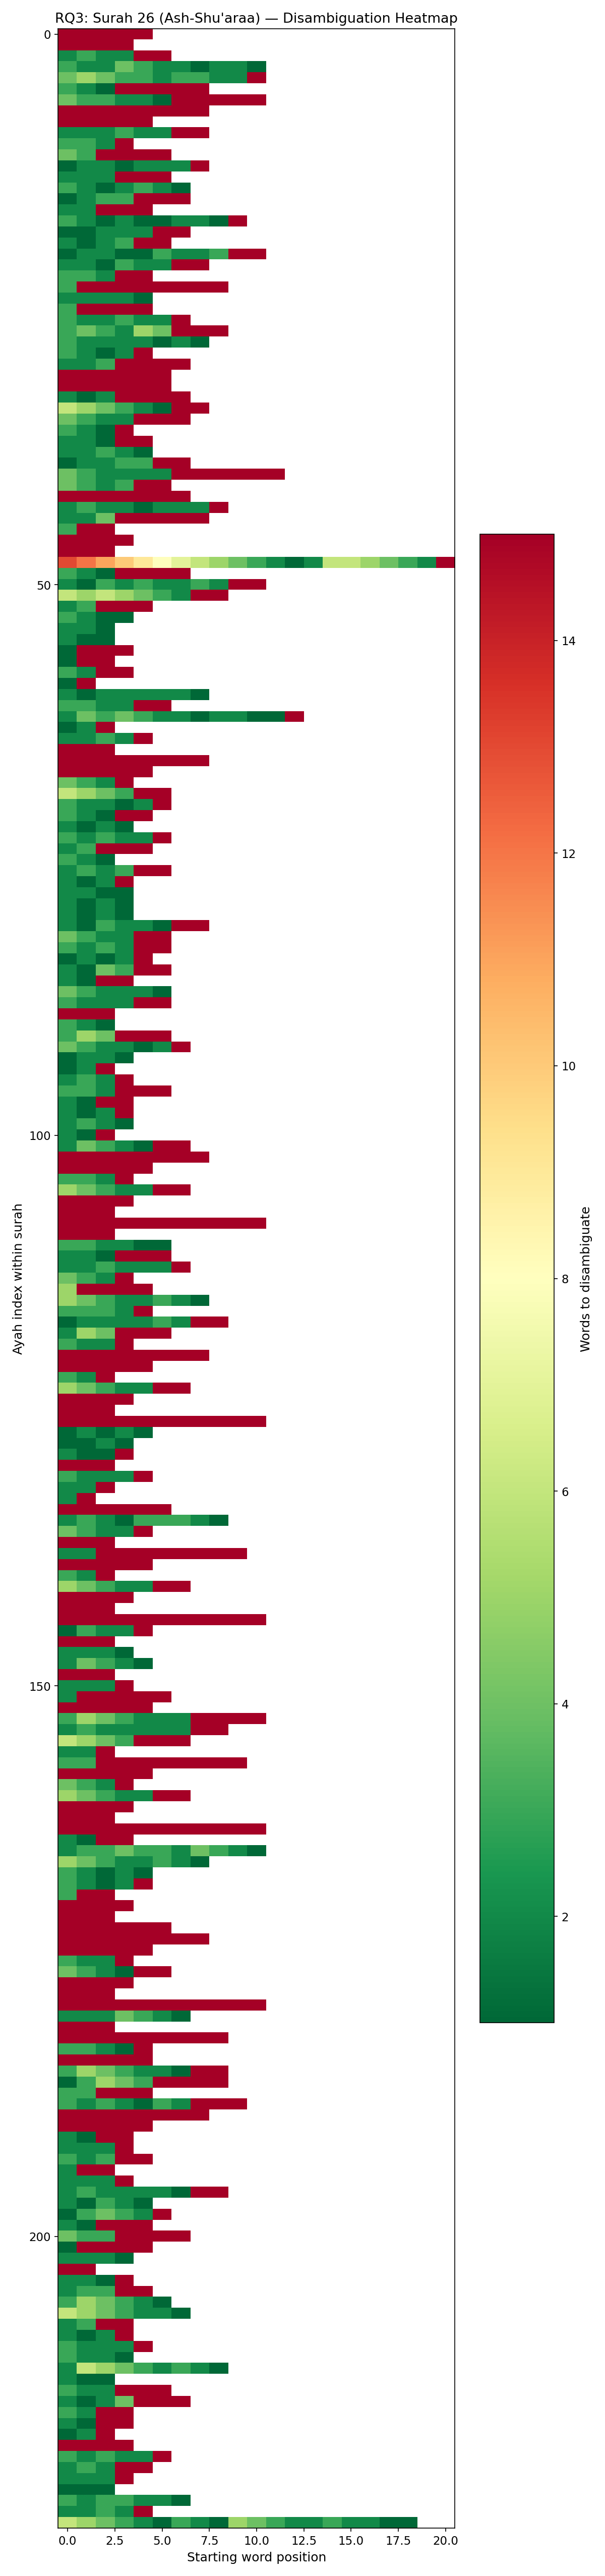
\includegraphics[width=0.75\columnwidth]{fig_10_heatmap_26.png}
  \caption{Surat al-Shu`ara' (Q\,26): periodic bands from repeated prophet-narrative structures.}
\end{figure}

\begin{figure}[h]
  \centering
  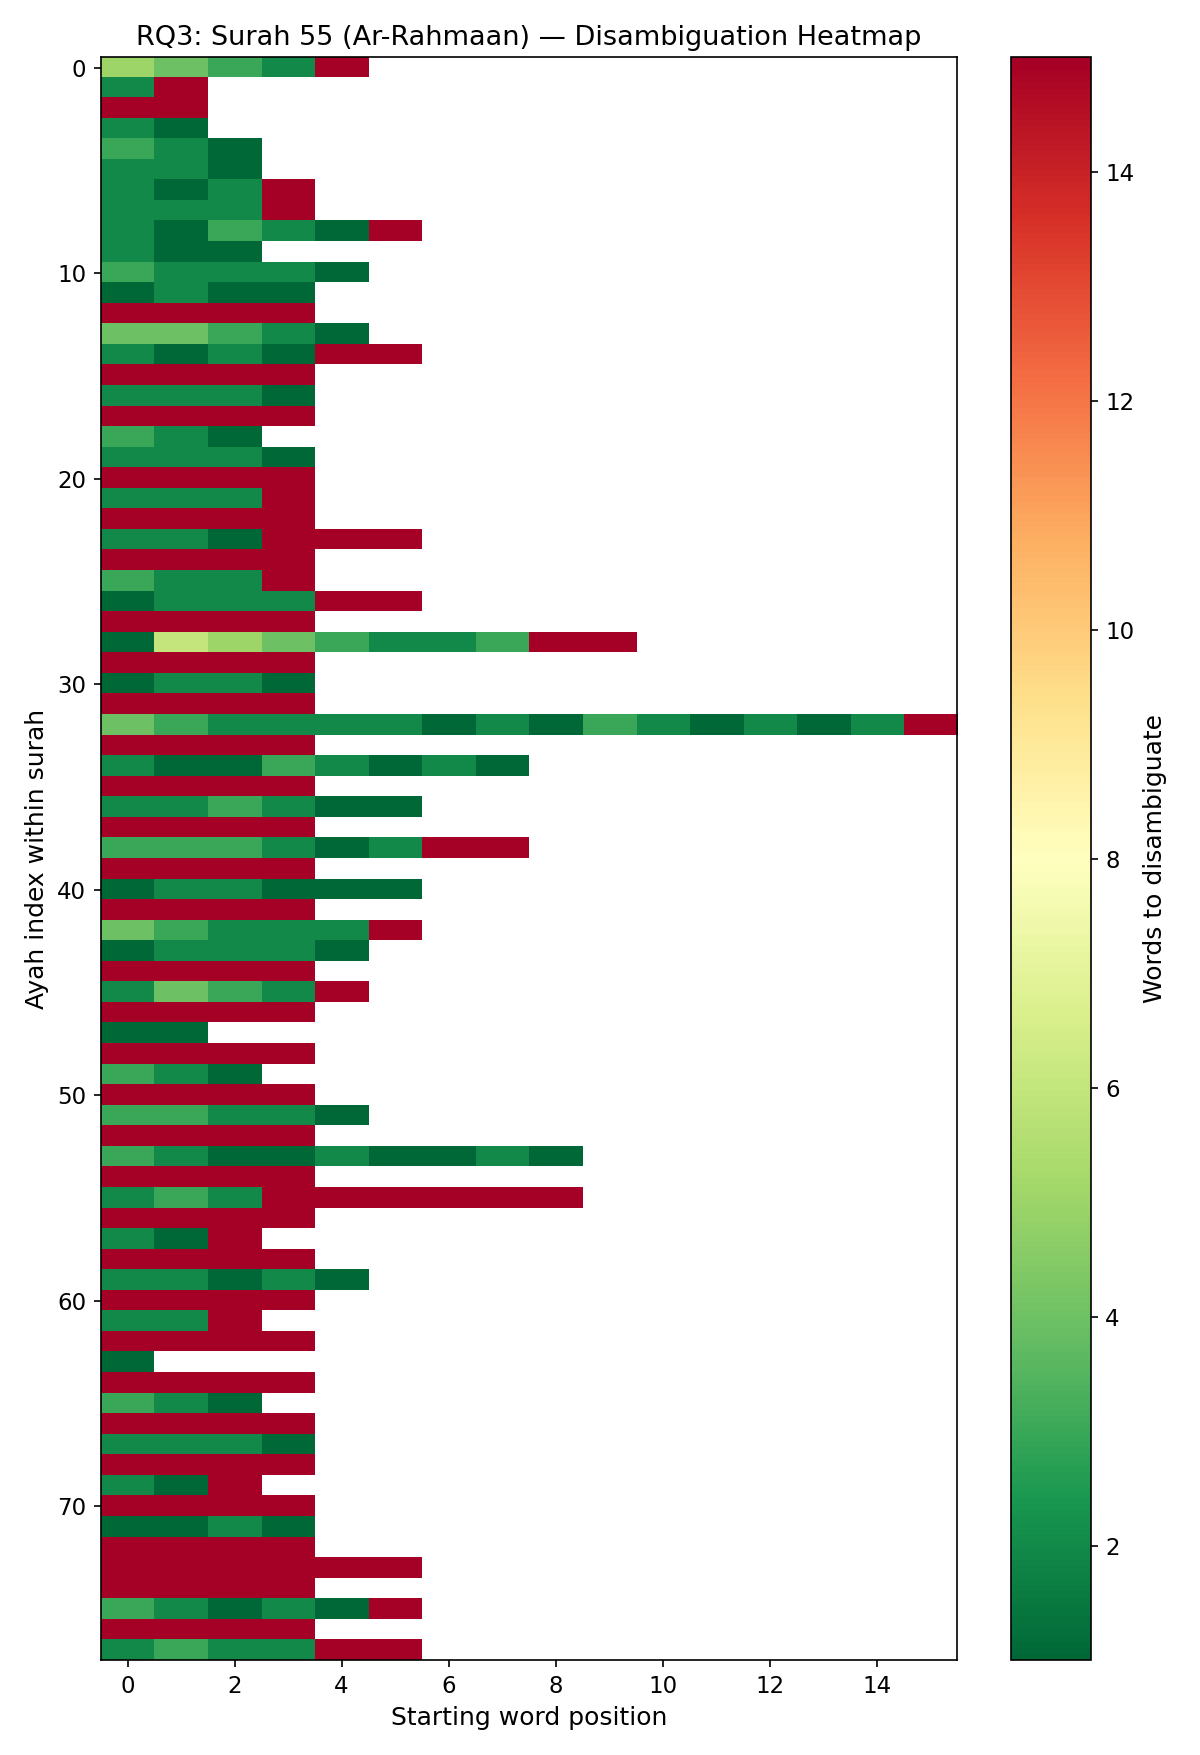
\includegraphics[width=0.75\columnwidth]{fig_11_heatmap_55.png}
  \caption{Surat al-Rahman (Q\,55): vertical bands from the 31-fold refrain.}
\end{figure}

\begin{figure}[h]
  \centering
  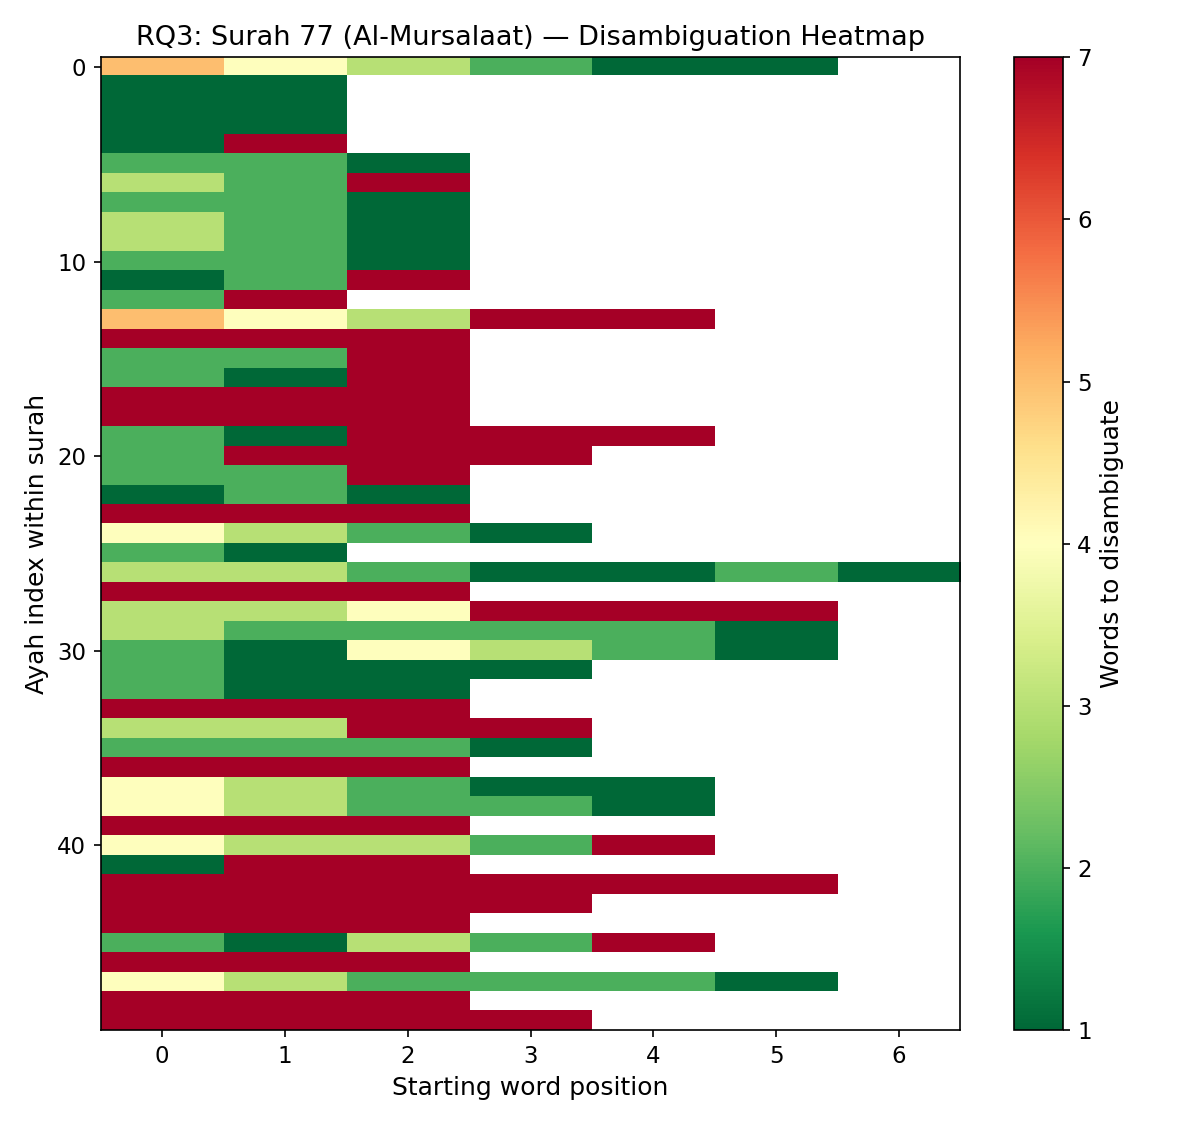
\includegraphics[width=0.75\columnwidth]{fig_12_heatmap_77.png}
  \caption{Surat al-Mursalat (Q\,77): banding from 10-fold refrain.}
\end{figure}

\begin{figure}[h]
  \centering
  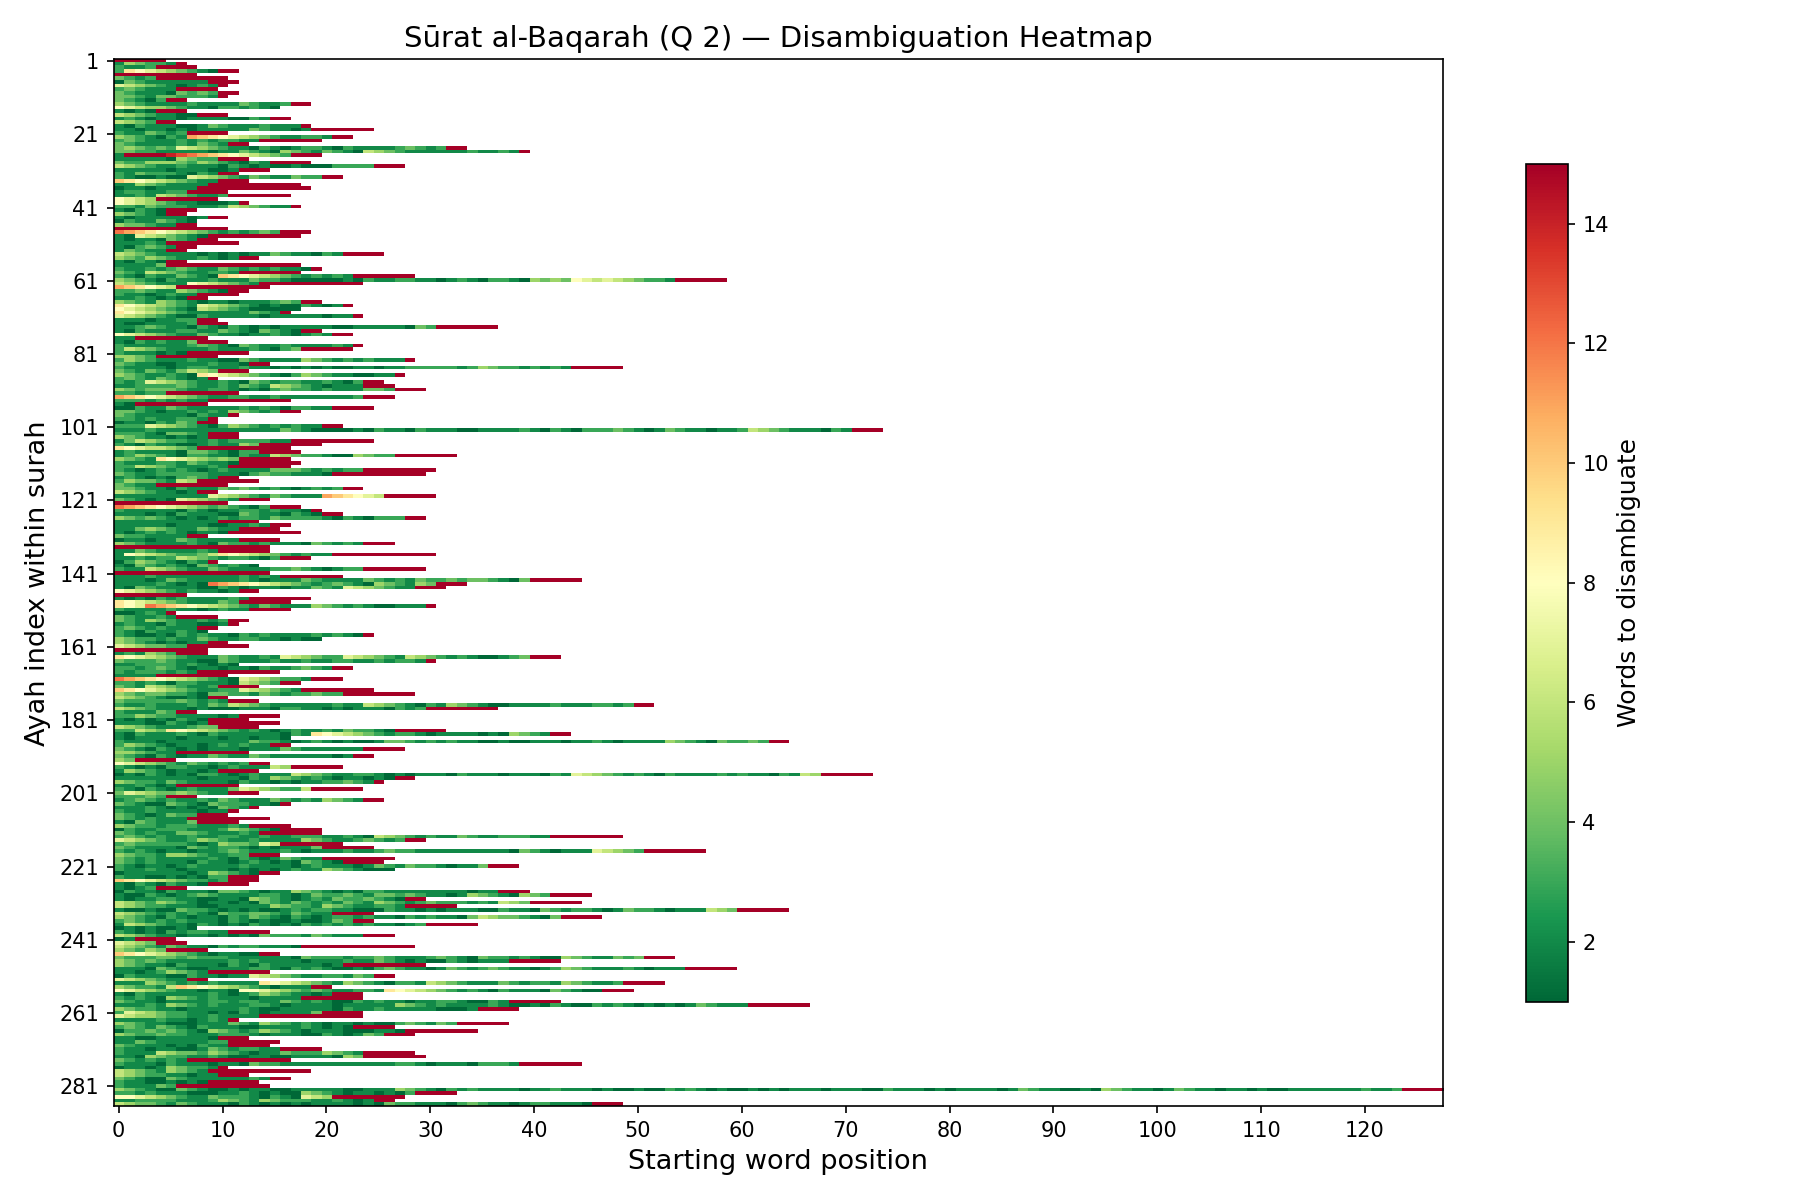
\includegraphics[width=0.75\columnwidth]{fig_13_heatmap_2.png}
  \caption{Surat al-Baqarah (Q\,2): 286 ayahs with scattered peaks.}
\end{figure}

\begin{figure}[h]
  \centering
  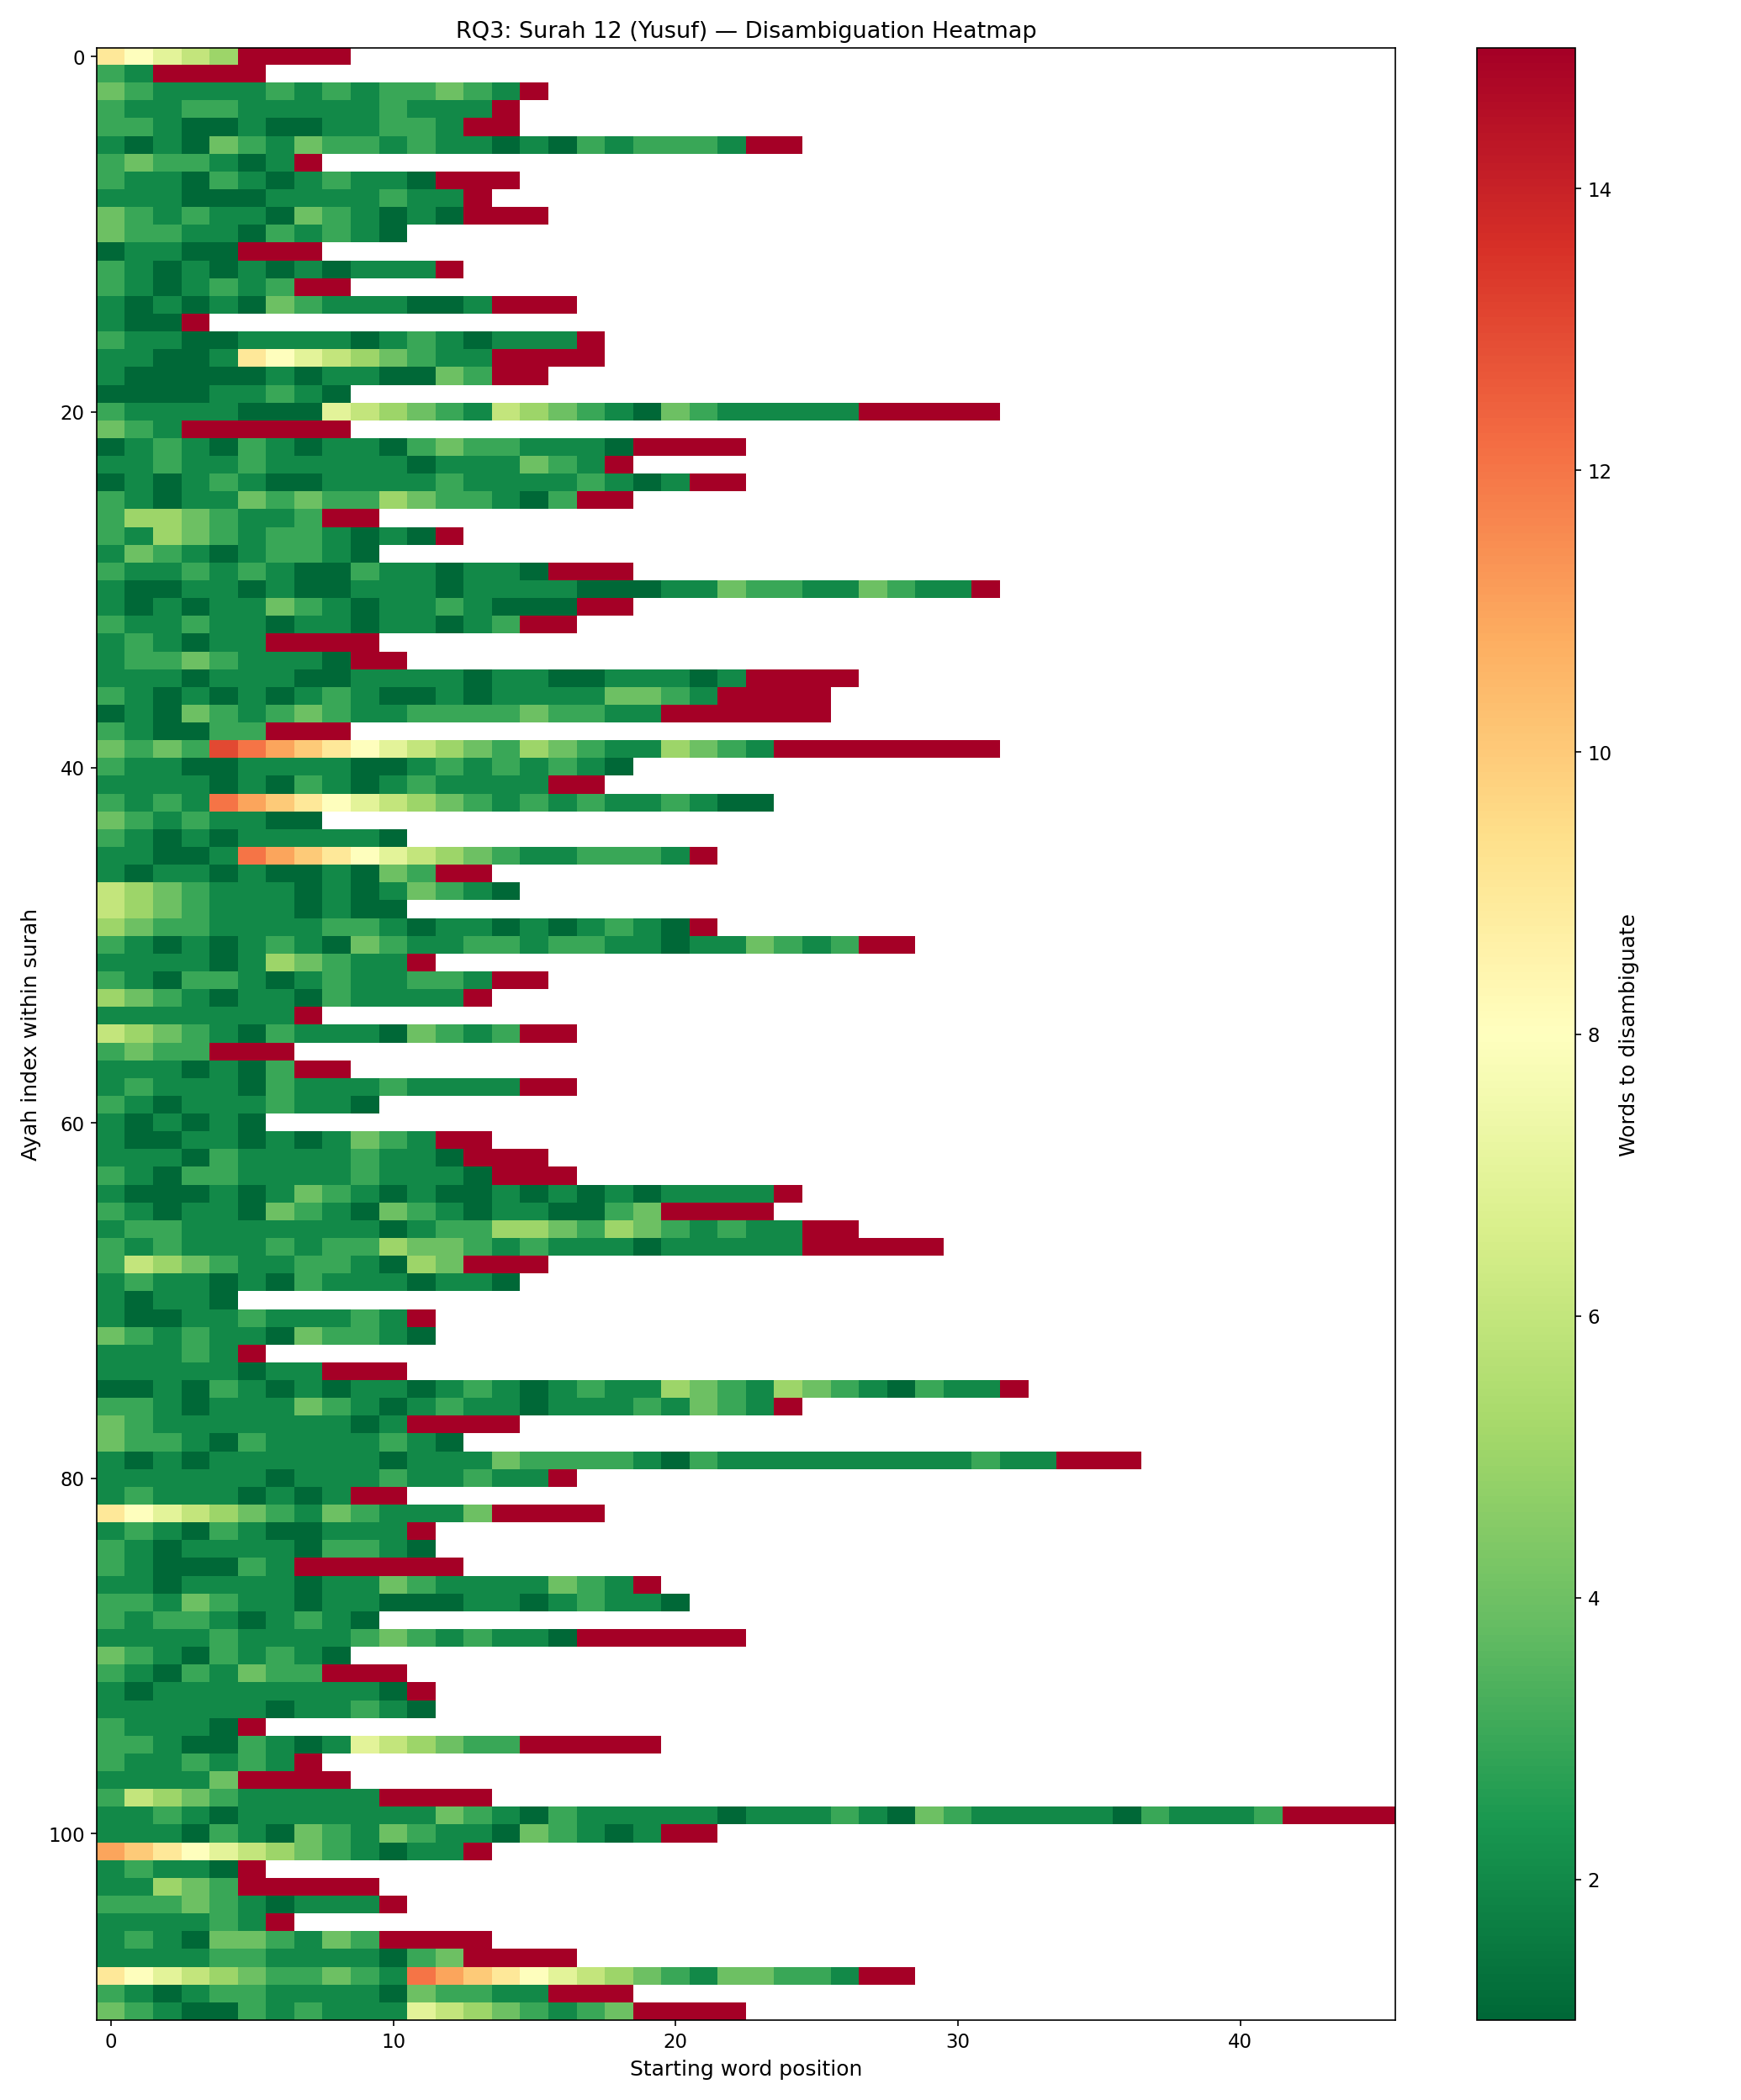
\includegraphics[width=0.75\columnwidth]{fig_14_heatmap_12.png}
  \caption{Surat Yusuf (Q\,12): a narrative surah with uniformly low difficulty.}
\end{figure}

\section{Top 10 Shared Closing Phrases}
\label{app:phrases}

\begin{table}[h]
\centering
\normalsize
\renewcommand{\arraystretch}{1.3}
\begin{tabular}{lcc}
\toprule
\textbf{Phrase} & \textbf{Freq.} & \textbf{NUR} \\
\midrule
\emph{ghaf\=urun ra\d{h}\=im} (Most Forgiving, Most Merciful) & 42 & 100\% \\
\emph{rabbu al-`\=alam\=in} (Lord of the Worlds) & 34 & 100\% \\
\emph{fa-bi-ayyi \=al\=a'i\ldots} (Which of your Lord's favors\ldots) & 31 & 100\% \\
\emph{al-`az\=izu al-\d{h}ak\=im} (the Almighty, the All-Wise) & 29 & 100\% \\
\emph{in kuntum \d{s}\=adiq\=in} (if you are truthful) & 28 & 100\% \\
\emph{all\=ahu ghaf\=urun ra\d{h}\=im} (God is Most Forgiving, Most Merciful) & 22 & 100\% \\
\emph{f\=ih\=a kh\=alid\=un} (therein they abide) & 19 & 100\% \\
\emph{al-qawm al-\d{z}\=alim\=in} (the wrongdoing people) & 19 & 100\% \\
\emph{m\=a k\=an\=u ya`mal\=un} (what they used to do) & 18 & 100\% \\
\emph{bi-kulli shay'in `al\=im} (Knower of all things) & 16 & 100\% \\
\bottomrule
\end{tabular}
\caption{Top 10 shared closing phrases. NUR = never-unique rate.}
\label{tab:phrases}
\end{table}

\section{Confuser Graph Statistics}
\label{app:graph}

\begin{table}[h]
\centering
\normalsize
\renewcommand{\arraystretch}{1.3}
\begin{tabular}{lr}
\toprule
\textbf{Metric} & \textbf{Value} \\
\midrule
Nodes ($\geq$5-word overlap) & 1{,}821 \\
Edges & 2{,}805 \\
Connected components & 429 \\
Largest component & 605 nodes \\
Max degree (Q\,2:255) & 38 \\
Cross-surah edges & 69.2\% \\
Symmetric persistent-confuser pairs & 677 \\
Cliff-then-plateau ayahs & 886 (14.2\%) \\
\bottomrule
\end{tabular}
\caption{Confuser graph statistics ($\geq$5 shared words).}
\label{tab:graph}
\end{table}

\section{Reproducibility}
\label{app:reproducibility}

The analysis requires Python 3.11+ with no external dependencies beyond the standard library.
The full pipeline completes in 6.5 seconds.
Given identical input, the output is \textbf{bit-for-bit identical} across runs and platforms.
All code and data: \url{[repository URL]}.

\end{document}